\chapter{A mixture-of-experts online learning system for adaptive behavior prediction}
\label{chap:mix_online_learning}

In this chapter, we continue our work on behavior prediction from chapter~\ref{chap:behav_pred}.
Although the various models developed there show already promising results, our analysis has shown, that each of the developed models has its own strengths and weaknesses in particular driving situations or even perform differently regarding the direction of motion (lateral or longitudinal) of the target vehicle.
Furthermore, they are intended to be trained offline and remain unchanged during deployment without any adaptation at run time.
Hence, relying on just one specific predictor would lead to sub-optimal performance in situations where one of the other models is superior.

Therefore, we investigate a mixture-of-experts online learning model to select between several offline trained models to achieve the best possible forecast.
Importantly, this model is intended to be trained online, i.e., continuously updating its weights based on the data received at run time.
This is one option to tackle the aforementioned issues with only one prediction model that has been trained offline before deployment.
By training a model at run time, we expect improved performance of the mixture model over the individual input predictors.
We aim to implement the online learning model to be independent of the type and number of prediction models used as input.
This enables the mixture model to either use several similar prediction models only differing in the encoding of the input data such as the \ac{LSTM}-based models in chapter~\ref{chap:behav_pred} or completely different models types such as one simple linear predictor and one simple single-layer neural network.
One of the advantages of such an approach is that instead of starting the model from a completely blank state, the individual predictors used as inputs for the mixture model already learned a consistent prior during their offline training.
Furthermore, the possibility of the offline models being validated in advance and serving as a fallback option in case the online model fails during deployment, is an additional advantage in a safety-critical domain such as automated driving.
Finally, the implementation of our approach employing the classic delta rule as well as the possibility to use spiking neuron models allows future deployment on dedicated neuromorphic hardware, which offers interesting possibilities regarding energy efficiency, especially in mobile applications and automotive context.
We investigate two different online learning systems differing in the information the model uses to optimize its weights.
In its simplest form, such a model adjusts its weight only based on the prediction error, i.e.\ the difference between its own prediction and the actual motion of the target vehicle.
However, we have seen in section~\ref{subsec:evaluation_of_the_lstm_based_prediction_models} that the performance of the individual models heavily depend on the current driving situation.
Therefore, we also investigate online learning models, that adjust their predictions based on some sort of contextual information.
We use the findings from section~\ref{subsec:evaluation_of_the_lstm_based_prediction_models} as a first hint regarding potential context information.

However, any online learning system making predictions about the future poses additional challenges.
For instance, the actual motion of the target vehicle and thus the error signal to update the neural weights is unknown at prediction time, but rather becomes available while the agent continues driving.
The temporally delayed error signal potentially introduces long lags between the prediction and the update of the corresponding weights.
Therefore, we need to find a mechanism to propagate the error between the actual,future motion of the target vehicle and the model's prediction back in time to update the weights correctly.
In this work, we address this issue through a temporal spreading of the error signal, i.e., we use the error of earlier prediction steps to update the weights of predictions further into the future.
Furthermore, we need to deal with the problem of over-fitting meaning that the model could just learn to predict the current vehicle particularly well but when switching to another vehicle with a potentially very different situational context and/or dynamics, the model's performance could deteriorate due to over-fitting the previous vehicle.
We evaluate our online learning model on real-world driving data and show, that the model is able to improve over the individual offline models already after being presented just a few vehicles.
Finally, while the type of online learning approach presented here has been shown to be successful in adaptive robot arm control \parencite{DeWolf2016}, to the best of our knowledge, our approach is the first trajectory prediction model to be trained during deployment for choosing from several pre-trained prediction models to achieve the best possible forecast.  


\section{Mixture-of-experts online learning models}%
\label{sec:instantiating_mixture_of_experts_online_learning_models}

In this section, we describe the architecture and learning rules of our proposed mixture-of-experts online learning models.
Importantly, all of the mixture-of-experts models shown in this chapter are meant to be trained \emph{online}.
That is, we do not pre-train them on a large corpus of data and then fix the final weights.
Instead, we run the neural network training \emph{while the system is running}.
We start with two variants of the model: one adapting its weights based solely on the prediction error and a more sophisticated model, which uses additional contextual information to adapt its neural weights.

\subsection{A context-free mixture-of-experts online learning model}%
\label{subsec:a_context_free_mixture_of_experts_online_learning_model}
\begin{figure}[t]
    \centering
    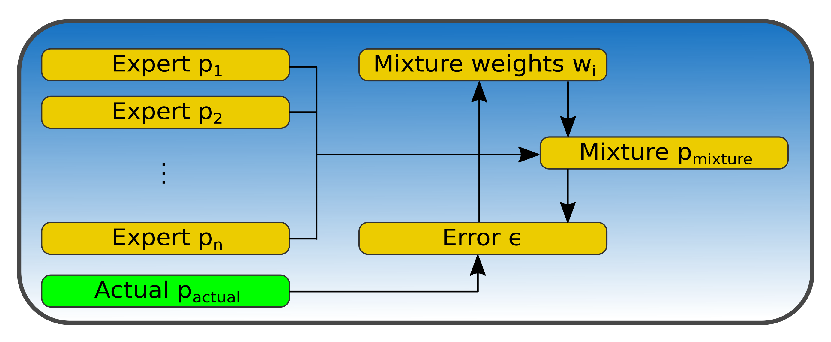
\includegraphics[width=0.8\linewidth]{imgs/mix_context_free_system_arch.eps}
    \caption{Visualization of the network architecture of the context-free mixture-of-experts online learning system with yellow boxes indicating the individual components of the model.
    The weights of the mixture-of-experts model depend solely on the error $\epsilon$ between the model's prediction and the actual future motion of the target vehicle.}
    \label{fig:mix_context_free_system_arch}
\end{figure}
Given that we have multiple models $ p_{i}$ for $i=1, \ldots, n$ predicting vehicle positions, we define the set of prediction models as 

\begin{equation}
\label{eq:mix_pred_model_set}
\mathcal{P} = \{ p_{i}  \quad | \quad i=1, \ldots, n \}.
\end{equation}

We construct our mixture-of-experts model in the following way.
We combine the predictions of the offline models using a simple weighted sum, and we use online training to learn these weights.
This core weighting algorithm is given by 

\begin{equation}
\label{eq:mix_weighting}
\mathbf{v}_{mix,t} = \sum\limits_{ p \in \mathcal{P}} \mathbf{W}_{ p ,t} \mathbf{v}_{ p ,t},
\end{equation}
where $\mathbf{v}_{ p ,t}$ is the predicted value for time $t$ into the future from offline model $p$, and $\mathbf{W}_{ p ,t}$ is the weight for expert $p$ for a prediction time of $t$.
Note that this means that the weighting between the expert predictions may be different depending on how far into the future we are predicting.
That is, in some conditions one expert should be weighted more highly than in other conditions, and we want to adapt this weighting based on experience.
Figure~\ref{fig:mix_context_free_system_arch} depicts the architecture of the context-free mixture-of-experts model variant with yellow boxes indicating the individual components of the model.

The weights $ \mathbf{W}_{ p ,t}$ are initialized equally over all predictors $ p$, i.e. $\mathbf{W}_{ p ,t} = 1/N_p$, where $N_p$ is the number of prediction models being combined, and then updated using online learning.
While any neural network learning algorithm could be used to do this, we adapt the classic delta learning rule, which is the basis of all gradient-descent learning algorithms, for the sake of simplicity and ease of implementation:

\begin{equation}
  \label{eq:mix_learning1}
\Delta\mathbf{W}_{p,t} = \kappa \nu_{t} \mathbf{v}_{p,t} \underbrace{(\mathbf{v}_{observed,t}-\mathbf{v}_{mix,t})}_{=\epsilon_t} = \kappa \nu_{t} \mathbf{v}_{p,t} \epsilon_t.
\end{equation}
where $\kappa$ is the learning rate and $\nu_{t}$ is a factor to scale the learning rate $\kappa$ differently for each prediction time step.

\subsection{A context-sensitive mixture-of-experts online learning model}%
\label{subsec:a_context_sensitive_mixture_of_experts_online_learning_model}

\begin{figure}[t!]
    \centering
    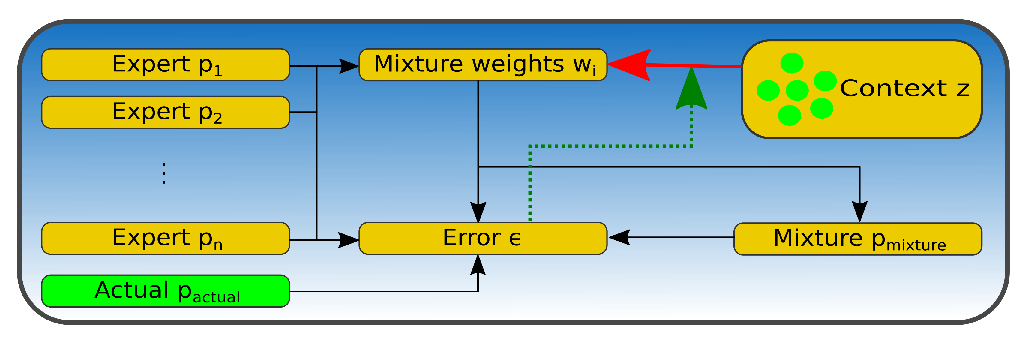
\includegraphics[width=\textwidth]{imgs/mix_system_arch.eps}
    \caption{Visualization of the network architecture of the context-sensitive mixture-of-experts online learning system.
    Yellow boxes indicate the individual components of the model, while the solid red line depicts the connection to decode out the weights $ \mathbf{W}_{p,t}$ for the individual expert predictors from the neural population encoding the context $\mathbf{z}$ as indicated by the green circles in the context component.
    The dotted green arrow indicates that the error signal is used to update the weights of this connection using delta-rule learning.}
    \label{fig:mix_context_sensitive_system_arch}
\end{figure}

The above model attempts to find the best weighting of the individual prediction models based solely on the prediction error or the mixture-of-experts model.
However, we believe that the ideal weights will crucially depend on some aspects of the current situation (i.e.\ the current context).
That is, instead of learning $ \mathbf{W}$, we can learn the function $f_{ \mathbf{W}}( \mathbf{z})= \mathbf{W}$, where $\mathbf{z}$ is some currently available sensor information.
Indeed, the context-free version shown in section~\ref{subsec:a_context_free_mixture_of_experts_online_learning_model} is equivalent to the context-sensitive models shown here if the context is kept constant.

Now our goal is to use this context information $\mathbf{z}$ to generate $\mathbf{W}$.
While any neural network learning algorithm could be used here, for simplicity we use a simple single hidden-layer neural network and adapt its weights by applying the delta rule again.
That is, we input the context values $\mathbf{z}$ into $N$ neurons (encoding), and the output of the network (decoding) will be the $\mathbf{W}$ values for the current context.
For this encoding and decoding, we use the principles of the \acf{NEF} as described in section~\ref{sec:neural_eng}.
The encoding process (the input weights for the neural network) is shown in equation~\eqref{eq:mix_encoding}, converting $\mathbf{z}$ into the activity $\mathbf{a}_i$ of the $i$th neuron:

\begin{equation}
  \mathbf{a}_{i} = \mathbf{G} \left(\sum_{j} \mathbf{e}_{i,j}\mathbf{z}_j+\beta_i\right)
  \label{eq:mix_encoding}
\end{equation}

$\mathbf{G}$ is the neuron non-linearity (here we use the rate-approximation of the Leaky Integrate and Fire neuron, although any other neuron model is likely to have similar behavior).
$\mathbf{e}_{i,j}$ and $\beta_i$ are randomly generated to produce a uniformly distributed range of maximum firing rates and intercepts (the $\mathbf{z}$ value at which the neuron starts firing), as per \textcite{Eliasmith2013}. 
This has been shown to be a good distribution of values for a wide variety of situations, and is consistent with what is observed in mammalian brains \parencite{Eliasmith2013}.
Unlike most neural network models, since these input weights are a reasonable distribution, we do not change $\mathbf{e}_{i,j}$ and $\beta_i$ at any time, leaving them at their initial randomly generated values.
In other words, we just adjust the weights between the hidden layer and the output layer, and leave the other set of weights at their initial randomly generated values.
This greatly reduces the computation cost of performing the online learning.

Given the neural activity $\mathbf{a}_i$ generated in equation~\eqref{eq:mix_encoding}, we now use 

\begin{equation}
  \mathbf{W}_{p,t} = \sum_{i} \mathbf{d}_{p,t,i}\mathbf{a}_i
  \label{eq:mix_decoding}
\end{equation}
to decode the $\mathbf{W}$ values for the current context $\mathbf{z}$. 
As with the context-free version of the model, we initialize the weights, i.e., here the $\mathbf{d}$ values such that there is an equal weighting across all the expert predictions, i.e., $\mathbf{W}_{p,t} = 1/N_p$ where $N_p$ is the number of prediction models being combined, for all context $\mathbf{z}$.
The $\mathbf{d}$ values achieving this equal weighting are found using least-squares minimization.

Now that we have this system for generating context-dependent weights, we can use online learning to adjust $\mathbf{d}$ to change the weights $\mathbf{W}$ based on the accuracy of the predictions. 
As with the context-free model variant, we use the delta learning rule given in equation~\eqref{eq:mix_learning1}  

\begin{equation}
    \tag{\eqref{eq:mix_learning1} revisited}
    \Delta\mathbf{W}_{p,t} = \kappa \nu_{t} \mathbf{v}_{p,t} \underbrace{(\mathbf{v}_{observed,t}-\mathbf{v}_{mix,t})}_{=\epsilon_t} = \kappa \nu_{t} \mathbf{v}_{p,t} \epsilon_t.
\end{equation}
that would determine how much to adjust $\mathbf{W}$ given the current error between the mixture-of-experts prediction and the observed actual position of the vehicle (i.e., the error in $\mathbf{v}$).  
$\kappa$ is the learning rate and $\nu_{t}$ is a factor to scale the learning rate $\kappa$ differently for each prediction time step.
However, rather than applying that change to $\mathbf{W}$ directly, we instead use that as the error signal for the delta rule applied to the decoding network, turning an adjustment to $\mathbf{W}$ into an adjustment to $\mathbf{d}$:
\begin{equation}
\Delta\mathbf{d}_{p,t,i} = \kappa \mathbf{a}_i \nu_{t} \mathbf{v}_{p,t} \epsilon_t = \mathbf{a}_i \Delta\mathbf{W}_{p,t}
  \label{eq:learning2}
\end{equation}
Figure~\ref{fig:mix_context_sensitive_system_arch} shows a schematic visualization of our model's architecture.
Yellow boxes indicate the individual components of the model, while the solid red line depicts the connection to decode out the weights $ \mathbf{W}_{p,t}$ for the individual expert predictors from the neural population encoding the context $\mathbf{c}$ as indicated by the green circles in the context component.
Finally, the dotted green arrow indicates that the error signal is used to update the weights of this connection using delta-rule learning.

\subsection{Temporal spreading of the error signal}%
\label{subsec:temporal_spreading_of_the_error_signal}

One extremely important consideration for any online updating of a predictive model (i.e., one where it is generating anticipated future observations) is that the error signal is only available in the future.
That is, we can only apply Equation~\eqref{eq:learning2} after the amount of time $t$ has occurred.  
This introduces a long lag into the learning process.  
We illustrate this issue using an example situation showing the predictions of the individual offline models depicted in figure~\ref{fig:mix_individual_predictors_example}.
In this example, all individual models predict the target vehicle's motion in $y$-direction almost perfectly until a prediction horizon of roughly \SI{2.5}{\second} when the predictions start to deviate from the actual motion.
Assuming a similar situation for a model employing an online learning approach, the weights for the current prediction \SI{2.5}{\second} into the future can only be updated after \SI{2.5}{\second} have passed. 
For all prediction time-steps further into the future, we have to wait even longer while the error between the prediction and the actual motion potentially increases even more.
In the meantime, the model is doomed to make predictions for these future time-steps based on sub-optimal weights based on past learning updates.
However, the example depicted in figure~\ref{fig:mix_individual_predictors_example} also hints, that the error at \SI{2.5}{\second} could already be used to update weights further into the future as, although the error increases, the general \emph{direction} of the deviation between predictions and actual motion remains the same. 
In other words, we assume that if our system is currently predicting too large a value at time $t$, then it is likely also to be predicting too large a value at time $ \tilde{t} > t$.
That is, whenever we have an observation at time $t$ that we compare with the prediction made $t$ time steps ago, we can also apply Equation~\eqref{eq:learning2} for all the larger values as well, i.e., we apply Equation~\eqref{eq:learning2} for all $ \tilde{t}$ with $ \tilde{t} > t$ once the amount of time $t$ has passed.
Since this is just an estimation, we want the predictions for time steps $ \tilde{t} $ further into the future than $t$ be less influenced by the error at $t$.
Hence, we exponentially scale down the amount of adjustment of $\mathbf{d}$ by the difference in time $ \tilde{t}-t$, leading to our final learning rule:

\begin{equation}
    \Delta\mathbf{d}_{p, \tilde{t} ,i} = \kappa \mathbf{a}_i \nu_{t} \mathbf{v}_{p,t} (\mathbf{v}_{observed,t}-\mathbf{v}_{mix,t}) e^{-{( \tilde{t} - t)}/\tau} ~~~~~~ \textrm{for all}~ \tilde{t}  \geq t.
  \label{eq:learning3}
\end{equation}

\section{Experiments and results}%
\label{sec:experiments_and_results}

In this chapter, we use the output of three different prediction models as input for our mixture-of-experts online learning model.
We use some of the models we developed and already evaluated in chapter~\ref{chap:behav_pred} as input to the mixture-of-experts model.
These individual predictors are a simple \emph{linear} prediction model based on a constant velocity assumption and two \ac{LSTM}-based neural networks, referred to as \emph{\acs{SPA}} and \emph{numerical}.
Those are the models presented in section~\ref{subsec:lstm_based_prediction_models} and evaluated in section~\ref{subsec:evaluation_of_the_lstm_based_prediction_models}.
The architecture of the \ac{LSTM} models, which was already depicted in figure~\ref{fig:lstm_arch}, consist of one encoder and one decoder cell each for sequence to sequence prediction.
The \ac{SPA} model used as input to the mixture-of-experts online learning model employs the convolutive power encoding of the input data as shown in equation~\eqref{eq:conv_power_enc}, while the \emph{numerical} model simply uses raw numerical values as input data (see also section

For training the model, we simulate online deployment by presenting the \ac{LSTM} models' predictions on the validation subsets to the system.
Thereby, the individual experts perform their prediction on previously unseen data samples.
We conduct individual simulation runs for each of both data-sets.

We present results from two variants of our mixture-of-experts model.
Firstly, we evaluate a simplified version, which applies Equation \eqref{eq:learning2} directly at prediction time assuming that the error signal, which is future data, is actually available already at prediction time. 
The benefit of this prior evaluation is two-fold: on the one hand, we get an impression what benefits can be expected from using context information over the context-free variant before employing the more sophisticated, timing-sensitive model.
On the other hand, a model having immediate access to the future error signal serves as an upper bound for the performance to be expected from models that have to deal with temporally delayed error signals. 
We present the results of this prior evaluation in section~\ref{subsec:comparing_timing_agnostic_context_free_and_context_sensitive_mixture_models}, whereas the evaluation of the model tackling temporally delayed error signals is shown in section~\ref{subsec:evaluation_of_the_context_sensitive_model_variant_with_temporal_spreading}.

All model variants in this chapter are implemented using the neural simulator Nengo \parencite{Bekolay2014}, which is typically used for constructing large-scale biologically realistic neural models \parencite{Eliasmith2013}, but also allows for traditional feed-forward artificial neural networks using either spiking or non-spiking neurons.
Here, we use the rate-approximation of the Leaky Integrate and Fire neuron, although we expect any other neuron model to have similar behavior.
Spiking neurons are of considerable interest for automotive applications due to the potential for reduced power consumption when deployed on dedicated neuromorphic hardware. 


\subsection{Data and preprocessing}%
\label{subsec:data_and_preprocessing}
\begin{figure}[th!]
    \centering
    \includegraphics[width=0.9\linewidth]{imgs/mix_individual_predictors_example.png}
    \caption{One example from the \emph{On-board} data-set depicting a particular driving situation as well as the predictions made by each individual offline model used as input for our mixture-of-experts model.
        The upper row shows images of the ego-vehicle's ob-board cameras.
        The middle row shows the trajectory data where the dots indicate the position of the vehicles and color-code the vehicle type (red=motorcycle, green=car, blue=truck, black=ego-vehicle), the solid blue and orange line show past and future motion of the target vehicle, the other colored lines visualize the predictions of the offline models whereas gray lines depict the other vehicles' motion.
        Finally, the lower row shows the absolute error between each offline model's prediction and the actual positions of the target vehicle.
    }
    \label{fig:mix_individual_predictors_example}
\end{figure}

In this section, we describe the data we use to train and evaluate our mixture-of-experts models.
We use the same data-sets already used in chapter~\ref{chap:behav_pred} and detailed in section~\ref{sec:data_preproc}.
Figure~\ref{fig:mix_individual_predictors_example} depicts one particular data sample from the \emph{On-board} data-set showing a lane change maneuver of the target vehicle.
The upper row shows the raw images from the ego-vehicle's front and rear camera to get an idea of the driving situation with the target vehicle highlighted by a red box.
The middle row of plots shows the corresponding trajectory data for that particular driving situation, i.e., the positions of the vehicles during the past \SI{5}{\second}, the actual future motion of the vehicles as well as the offline model's predictions of the target vehicle's future motion.
The lower row finally shows the error between each model's prediction and the target vehicle's actual future motion for longitudinal ($x$) and lateral ($y$) direction separately.

\subsubsection{Input to the mixture model}%
\label{ssubsec:input_to_the_mixture_model}


Independent of what type of prediction model shown in chapter~\ref{chap:behav_pred} we use as input for the online learning system, the output of each individual predictor is anticipated positions in $x$- and $y$-direction at \num{20} equidistant time steps $t_i$ for $i=1,\ldots,20$ for \SI{5}{\second} into the future, i.e.\ $t_1=0.25, t_2=0.5, \ldots, t_{20}=5.0$.
Figure~\ref{fig:mix_individual_predictors_example} shows one data sample from the \emph{On-board} data-set depicting the input data to the offline models (previous motion) as well as each model's individual predictions, which are the input to the mixture model. 
In other words, the colored lines in figure~\ref{fig:mix_individual_predictors_example} depicting the predictions of the \emph{linear}, \emph{\ac{SPA}} and \emph{numerical} models form the input of the mixture-of-experts online learning model.
Note that these anticipated positions are each individual model's guesses about the actual position values used as ground truth in chapter~\ref{chap:behav_pred}.
We use these prediction values unaltered and without further preprocessing as input for our mixture models.
Furthermore, we only present vehicles from the test sets $V_1$ and $V_2$ to our mixture models to avoid presenting vehicles to the system the individual predictors have already been trained on.

\subsubsection{Contextual information used in the mixture model}%
\label{ssubsec:contextual_information_used_in_the_mixture_model}

In contrast to the anticipated positions predicted by each offline model we use as input to our mixture-of-experts model as described in the previous section, here we present the information used to describe the current driving situation, i.e., the contextual information encoded in the context population of our model.
While the context information used for the context-sensitive model variants could be described in many different ways, we use the following three pieces of information:

\begin{itemize}
    \item{$\mathbf{z}_1$: the current distance from the car to the ego-vehicle if available (note that there is no ego-vehicle the \ac{NGSIM} data-set. See section~\ref{subsec:ngsim-dataset})}
\item{$\mathbf{z}_2$: the current distance from the car to the nearest other car (including
    the ego-vehicle if available)}
\item{$\mathbf{z}_3$: the number of cars currently visible within a certain distance to the target vehicle}
\end{itemize}

We use the results from chapter~\ref{chap:behav_pred} as hint, since these pieces of information showed significant alterations depending on which prediction model performs best on the corresponding samples.
To translate these context values to a common order of magnitude, we use the training data to normalize these values and use their z-scores.

\subsection{Comparing timing-agnostic context-free and context-sensitive mixture models}%
\label{subsec:comparing_timing_agnostic_context_free_and_context_sensitive_mixture_models}

\begin{figure}[t]
    \centering
    \subfloat[\label{subfig:mix_start_on_board}]{%
        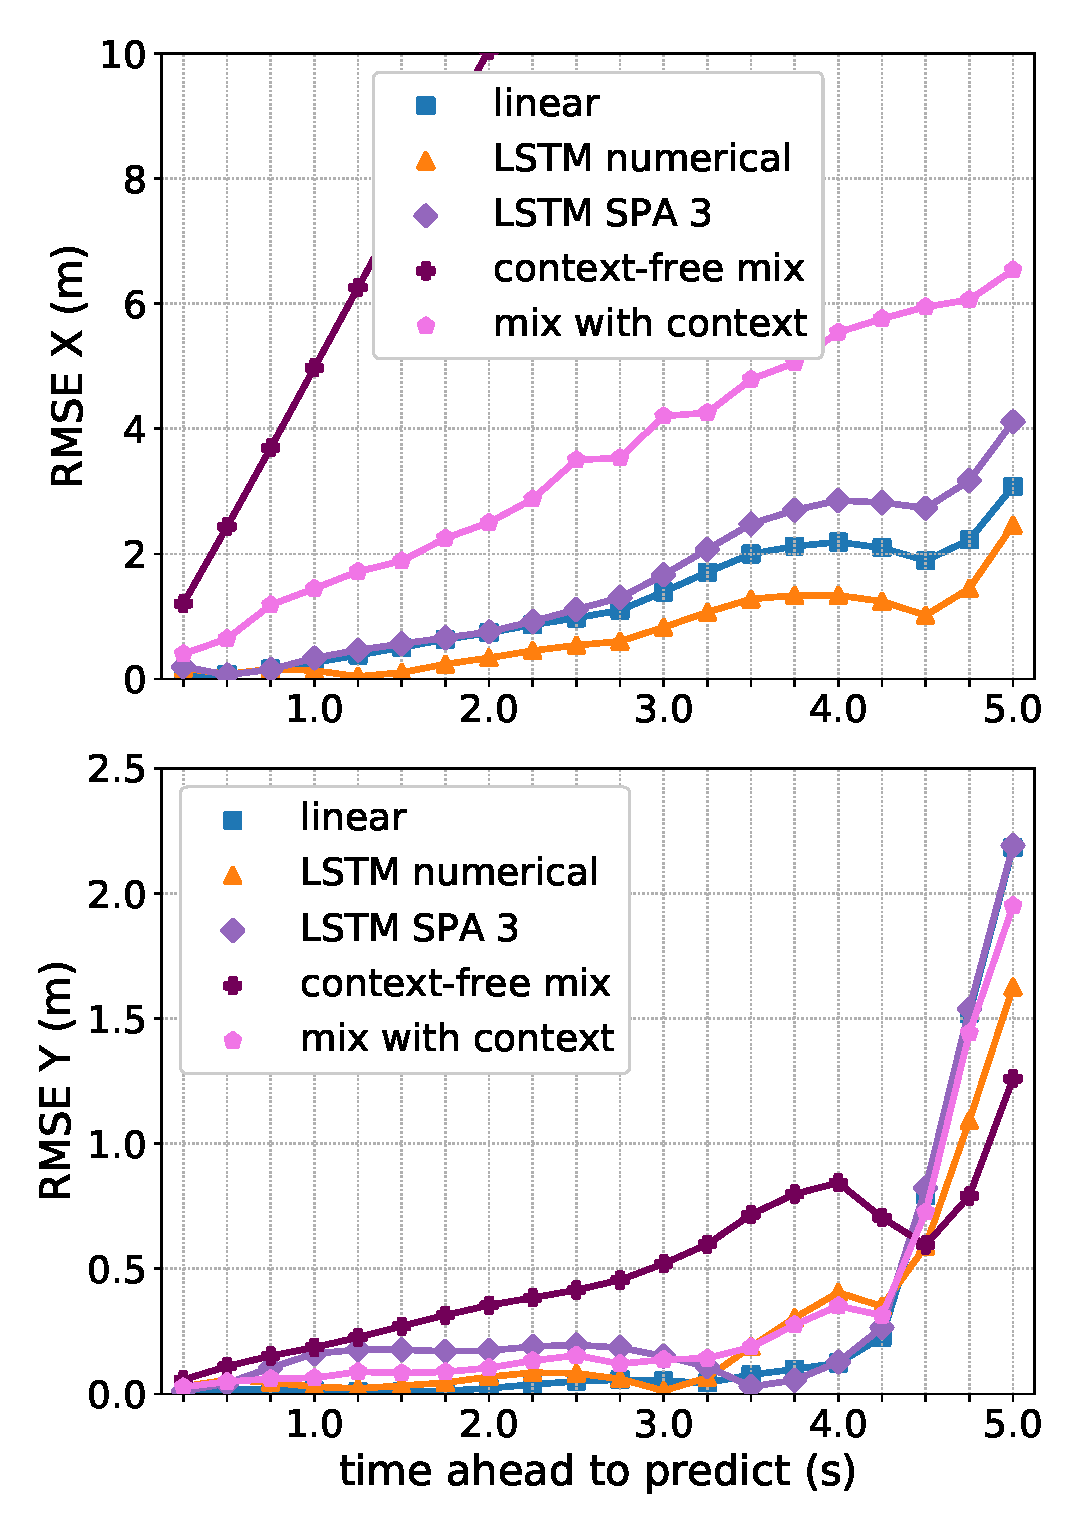
\includegraphics[width=0.25\linewidth]{imgs/mix_start_on_board.eps}
    }
    \subfloat[\label{subfig:mix_on_board}]{%
        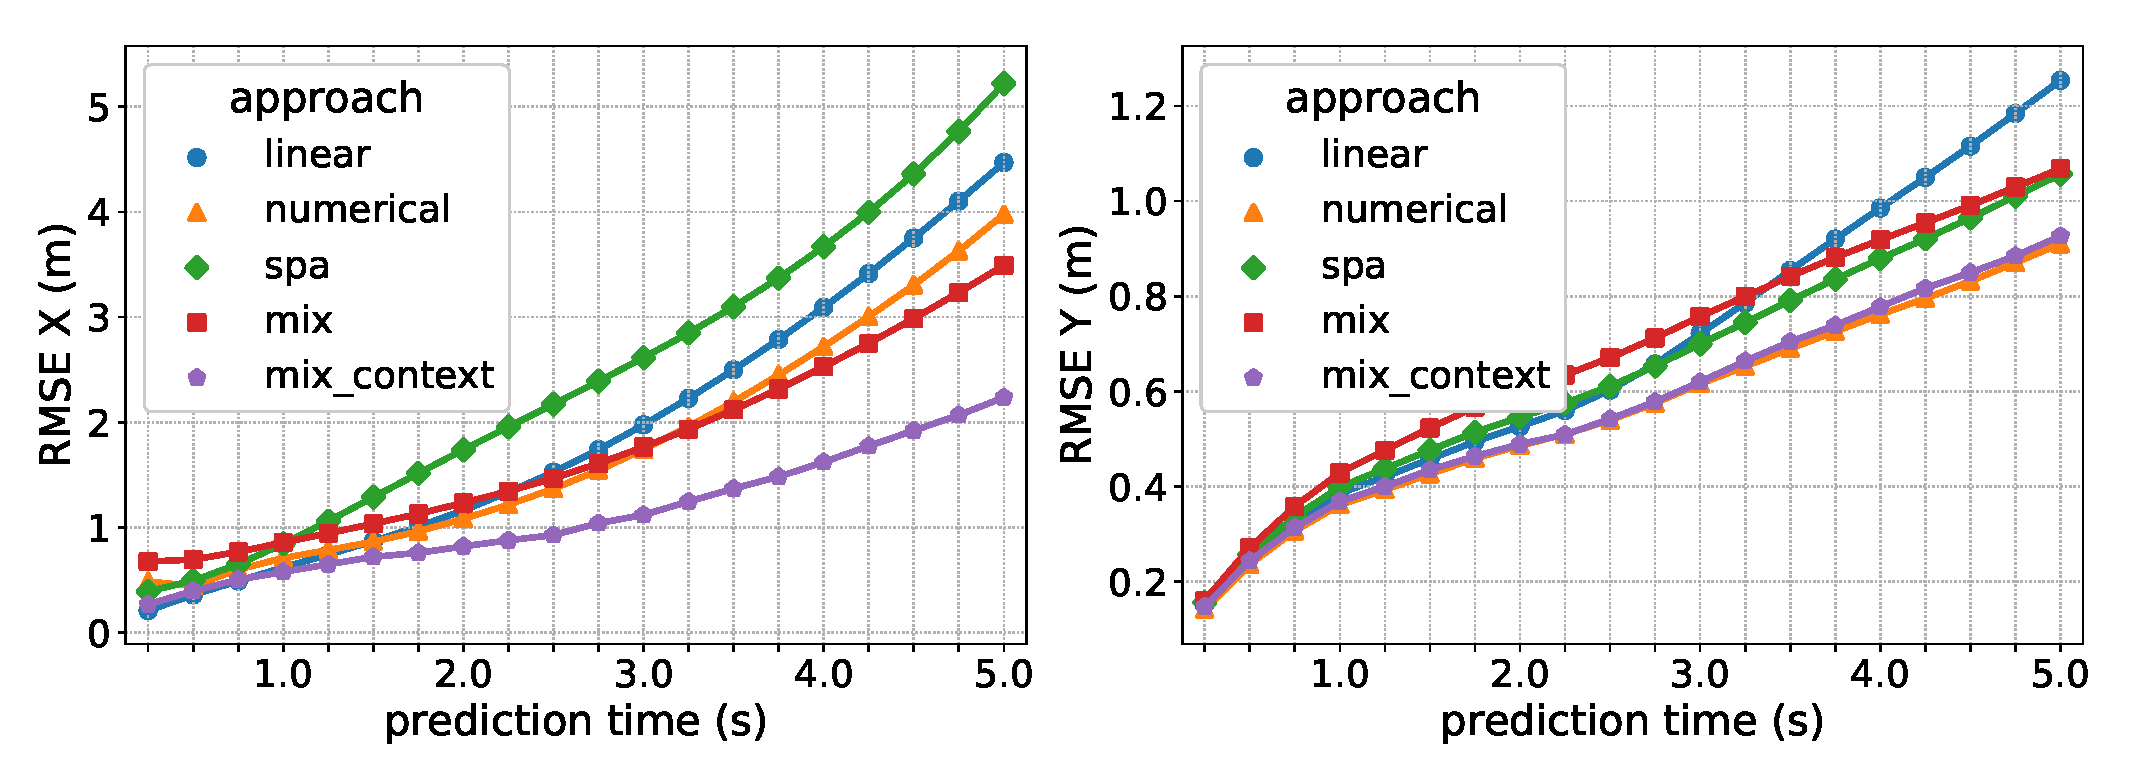
\includegraphics[width=0.25\linewidth]{imgs/mix_on_board.eps}
    }
    \subfloat[\label{subfig:mix_start_ngsim}]{%
        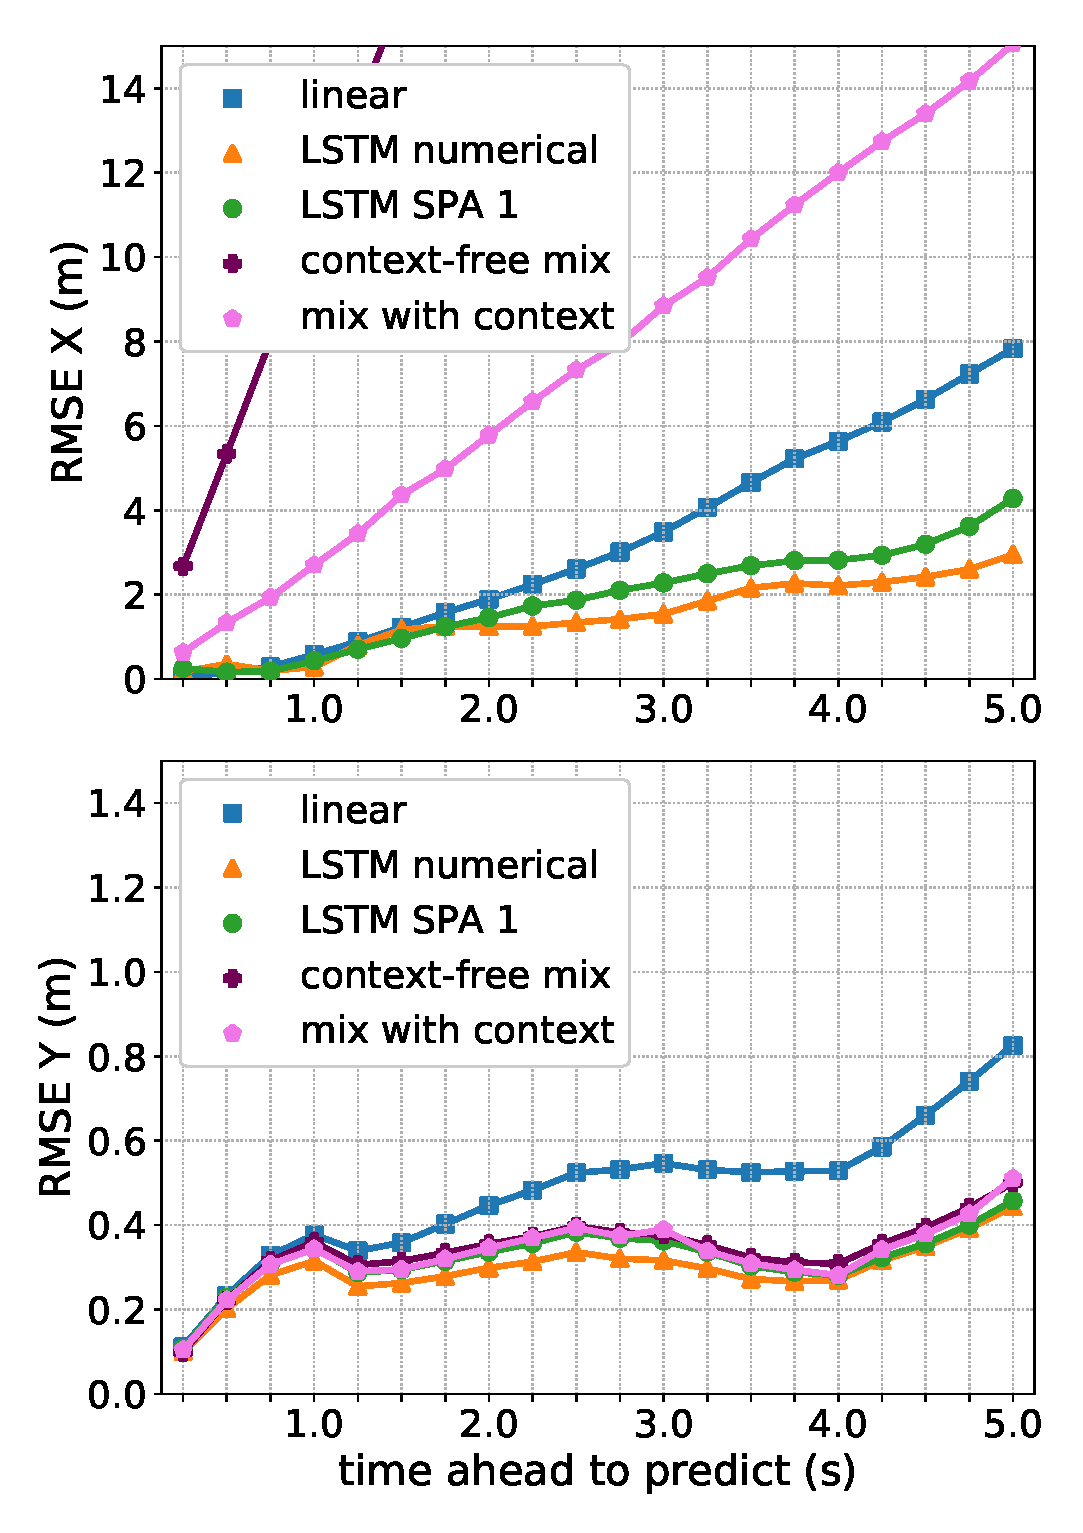
\includegraphics[width=0.25\linewidth]{imgs/mix_start_ngsim.eps}
    }
    \subfloat[\label{subfig:mix_ngsim}]{%
        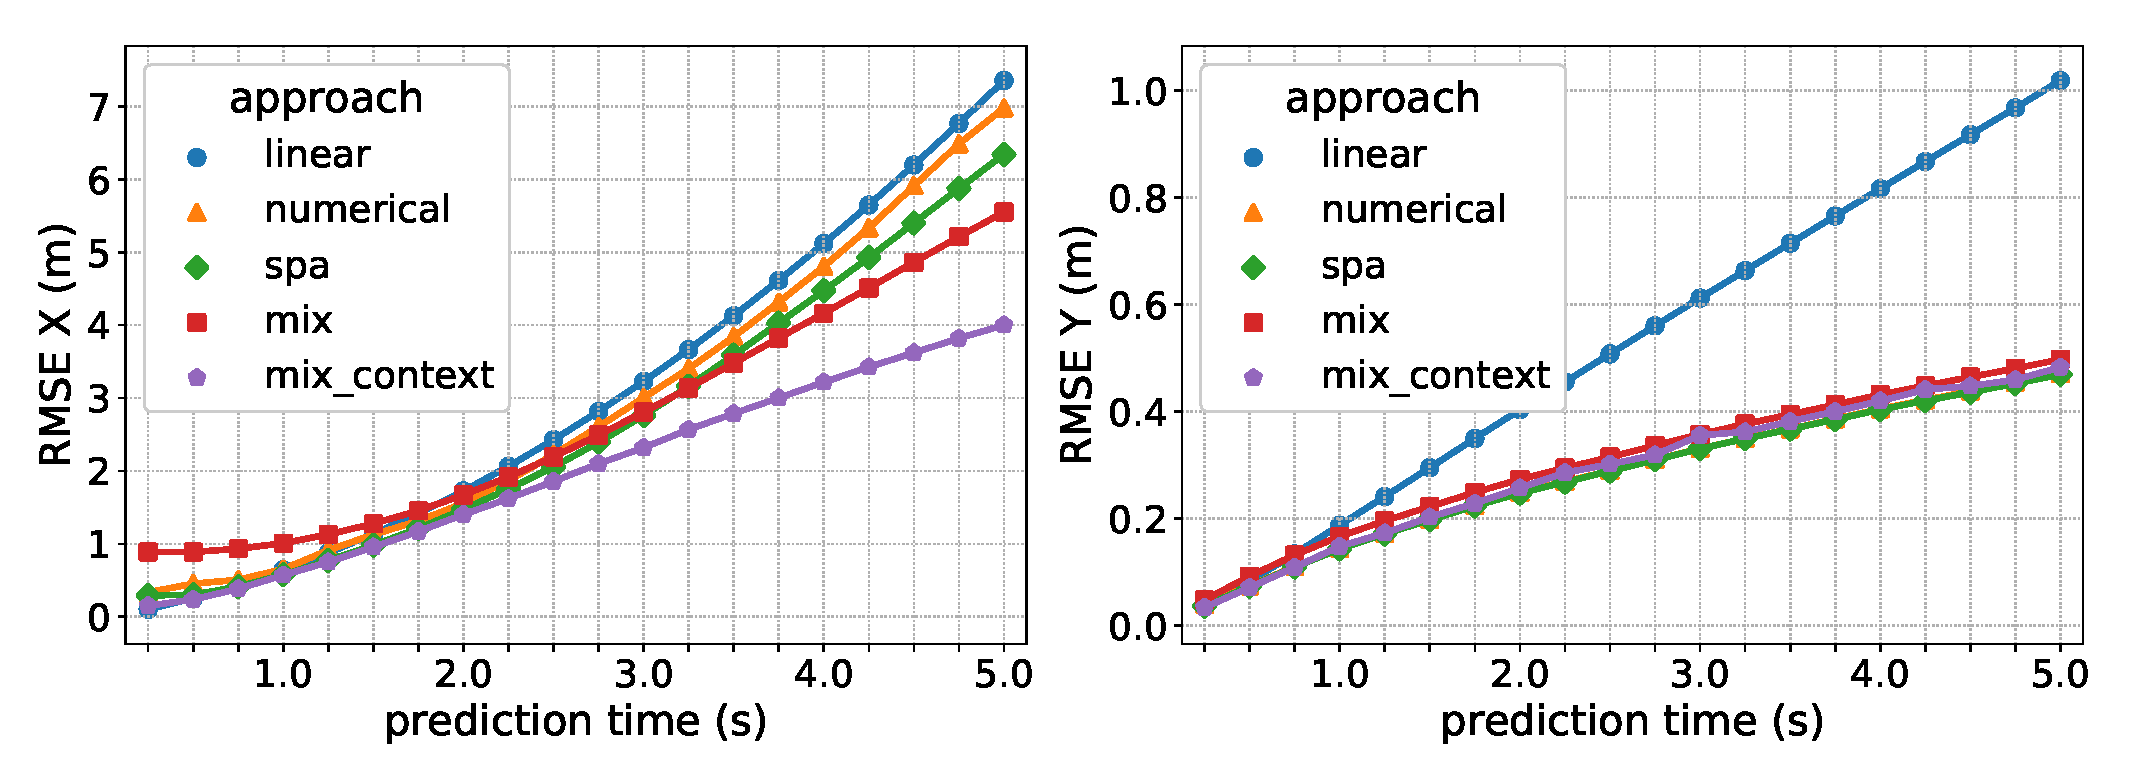
\includegraphics[width=0.25\linewidth]{imgs/mix_ngsim.eps}
    }
    \caption{Visualization of the \ac{RMSE} of the timing-agnostic variants of our mixture-of-experts model, both context-free and context-sensitive, on both data sets.
~\protect\subref{subfig:mix_start_on_board} shows the performance at the start of the training process on the \emph{On-board} data set. 
~\protect\subref{subfig:mix_start_ngsim} shows the performance at the start of the training process on the \emph{\ac{NGSIM}} data set. Similarly,~\protect\subref{subfig:mix_on_board} shows the models' performance on the first \num{70} vehicles of the \emph{on-board} data set, whereas figure~\protect\subref{subfig:mix_ngsim} show the models' performance on the first \num{92} vehicles of the \emph{\ac{NGSIM}} data set.}
    \label{fig:mix_timing_agnostic}
\end{figure}

In this section, we evaluate a simplified version of our mixture-of-experts online learning model, which ignores the fact, that the actual vehicle motion and thus the error signal for the weight updates is not available at prediction time.
Instead, we assume that Equation~\eqref{eq:learning2} can be applied directly at prediction time to update the weights without having to wait for the actual data to become available.
Thereby, we get an impression of the benefits that can be expected, if any, from using context information over the context-free variant before employing the more sophisticated, timing-sensitive model.
Furthermore, a model having immediate access to the future error signal serves as an upper bound for the performance to be expected from models that have to deal with temporally delayed error signals (see Section~\ref{subsec:evaluation_of_the_context_sensitive_model_variant_with_temporal_spreading}). 

\subsubsection{Experimental setup}%
\label{ssubsec:experimental_setup}

\begin{figure}[t!]
    \centering
    \subfloat[\label{subfig:mix_train_0_2} Predictions for first training vehicle \SI{0.75}{\second} into the future]{%
        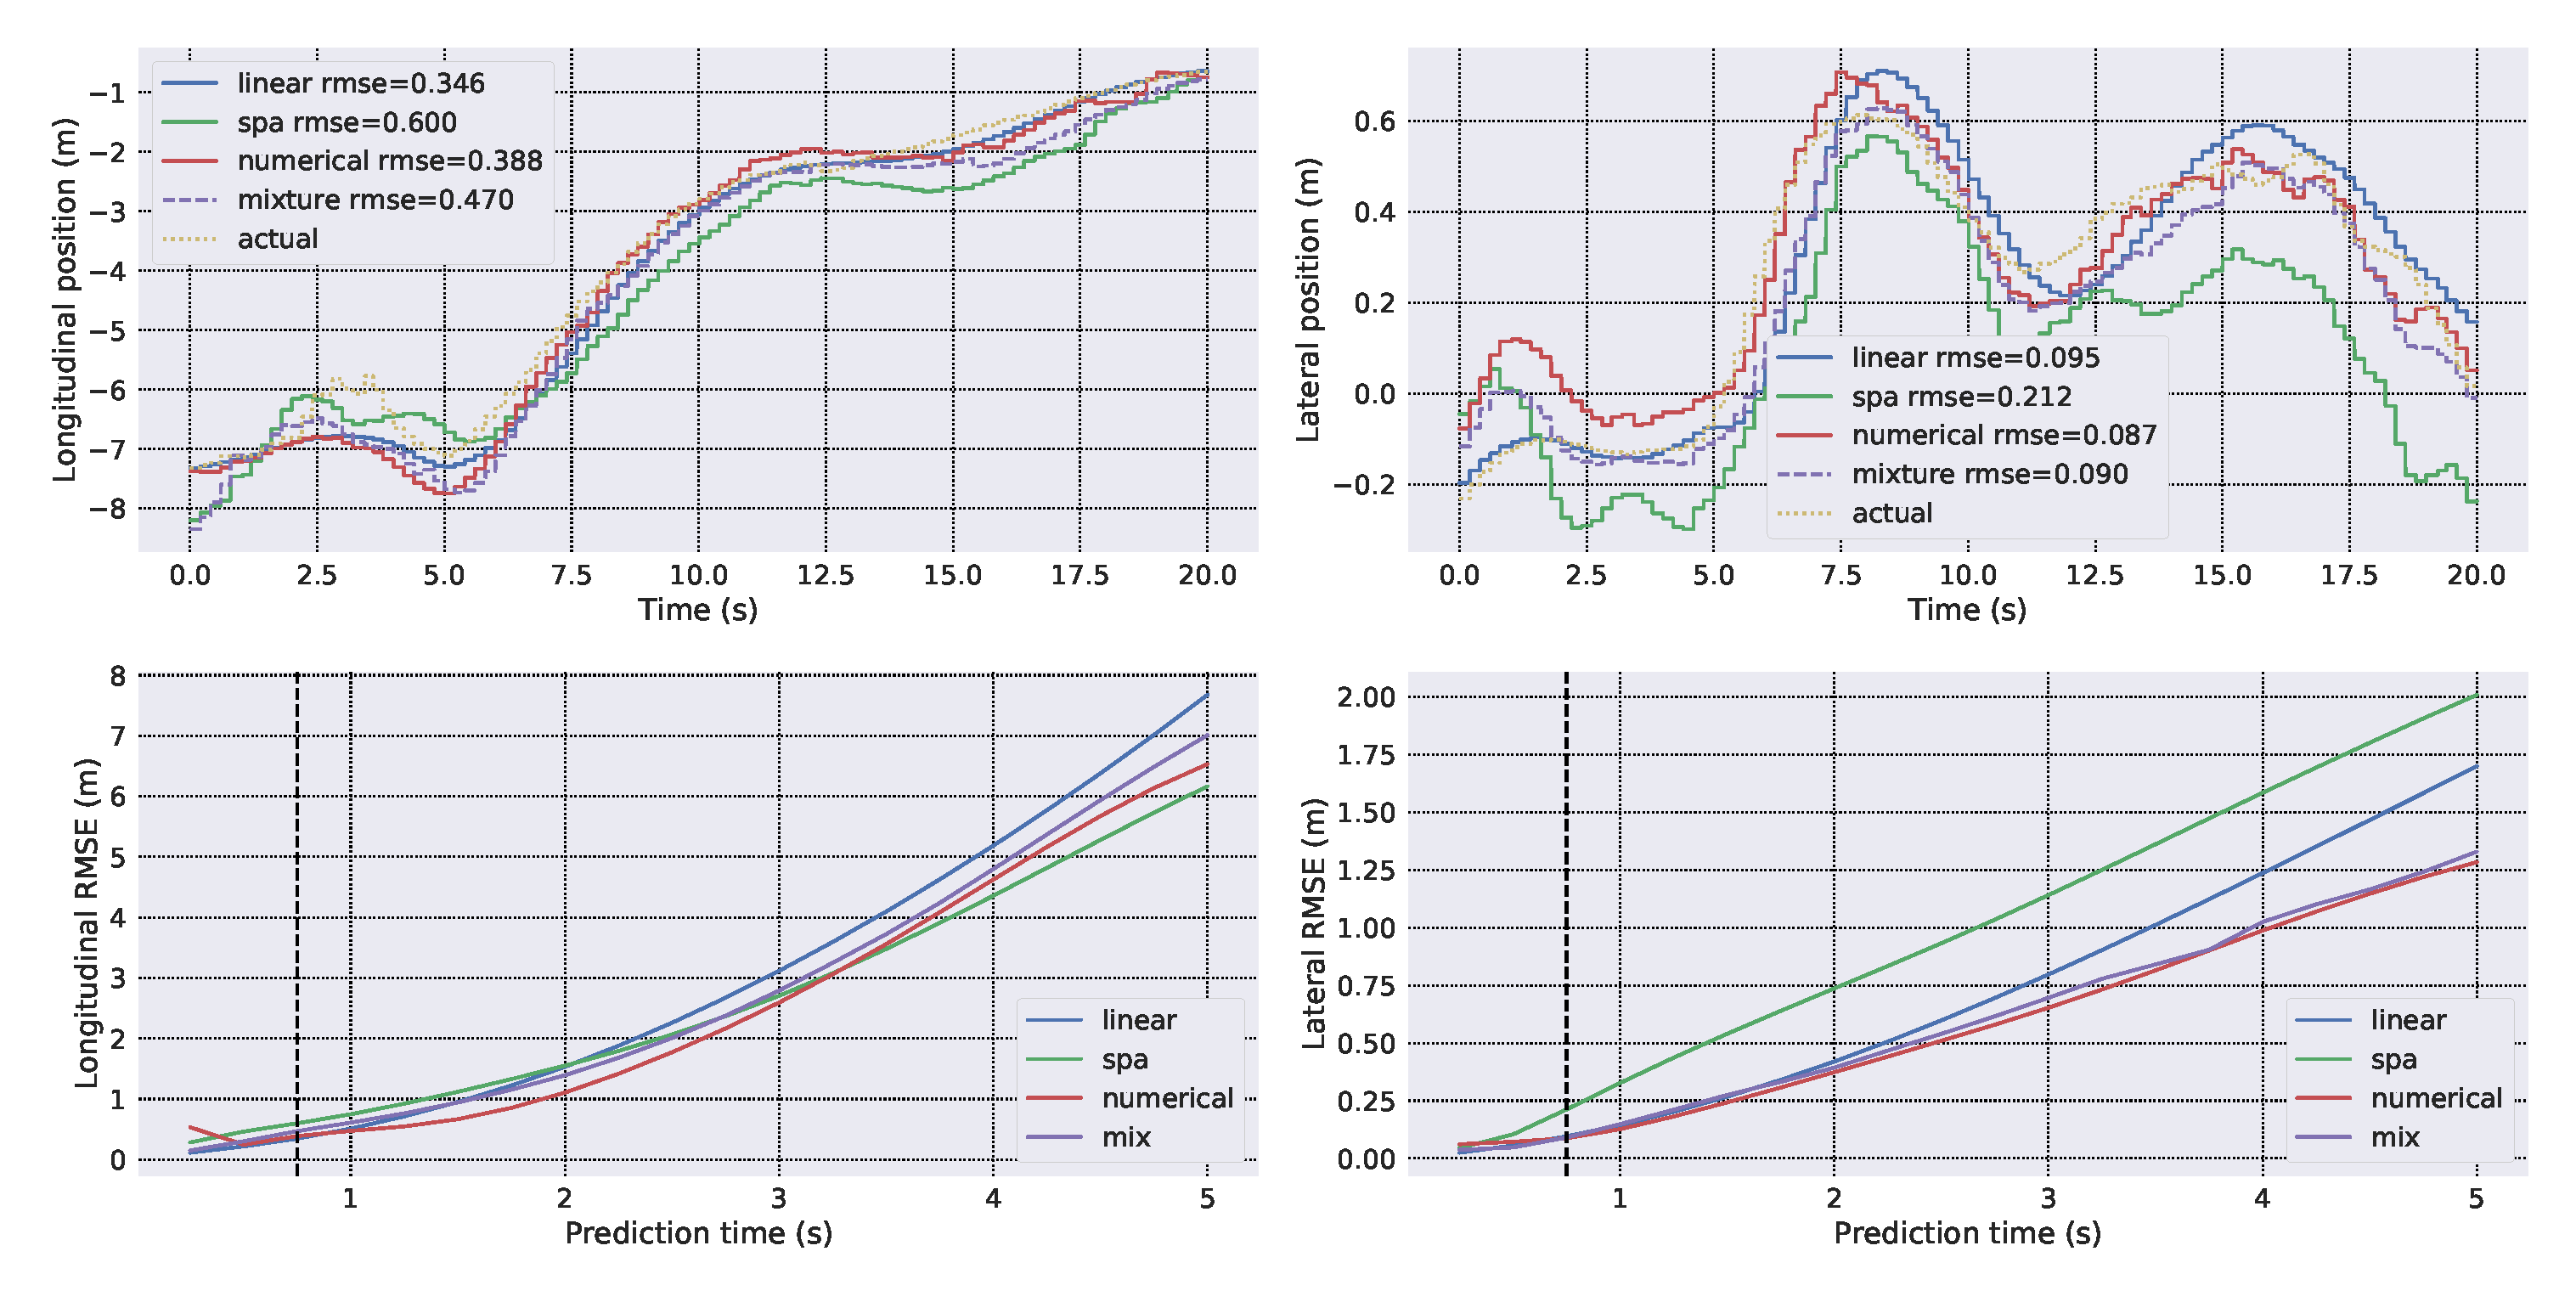
\includegraphics[width=0.8\linewidth]{imgs/mix_train_0_2.eps}
    }
    \vspace{-0.5cm}
    \subfloat[\label{subfig:mix_train_0_18}Predictions for first training vehicle \SI{4.75}{\second} into the future]{%
        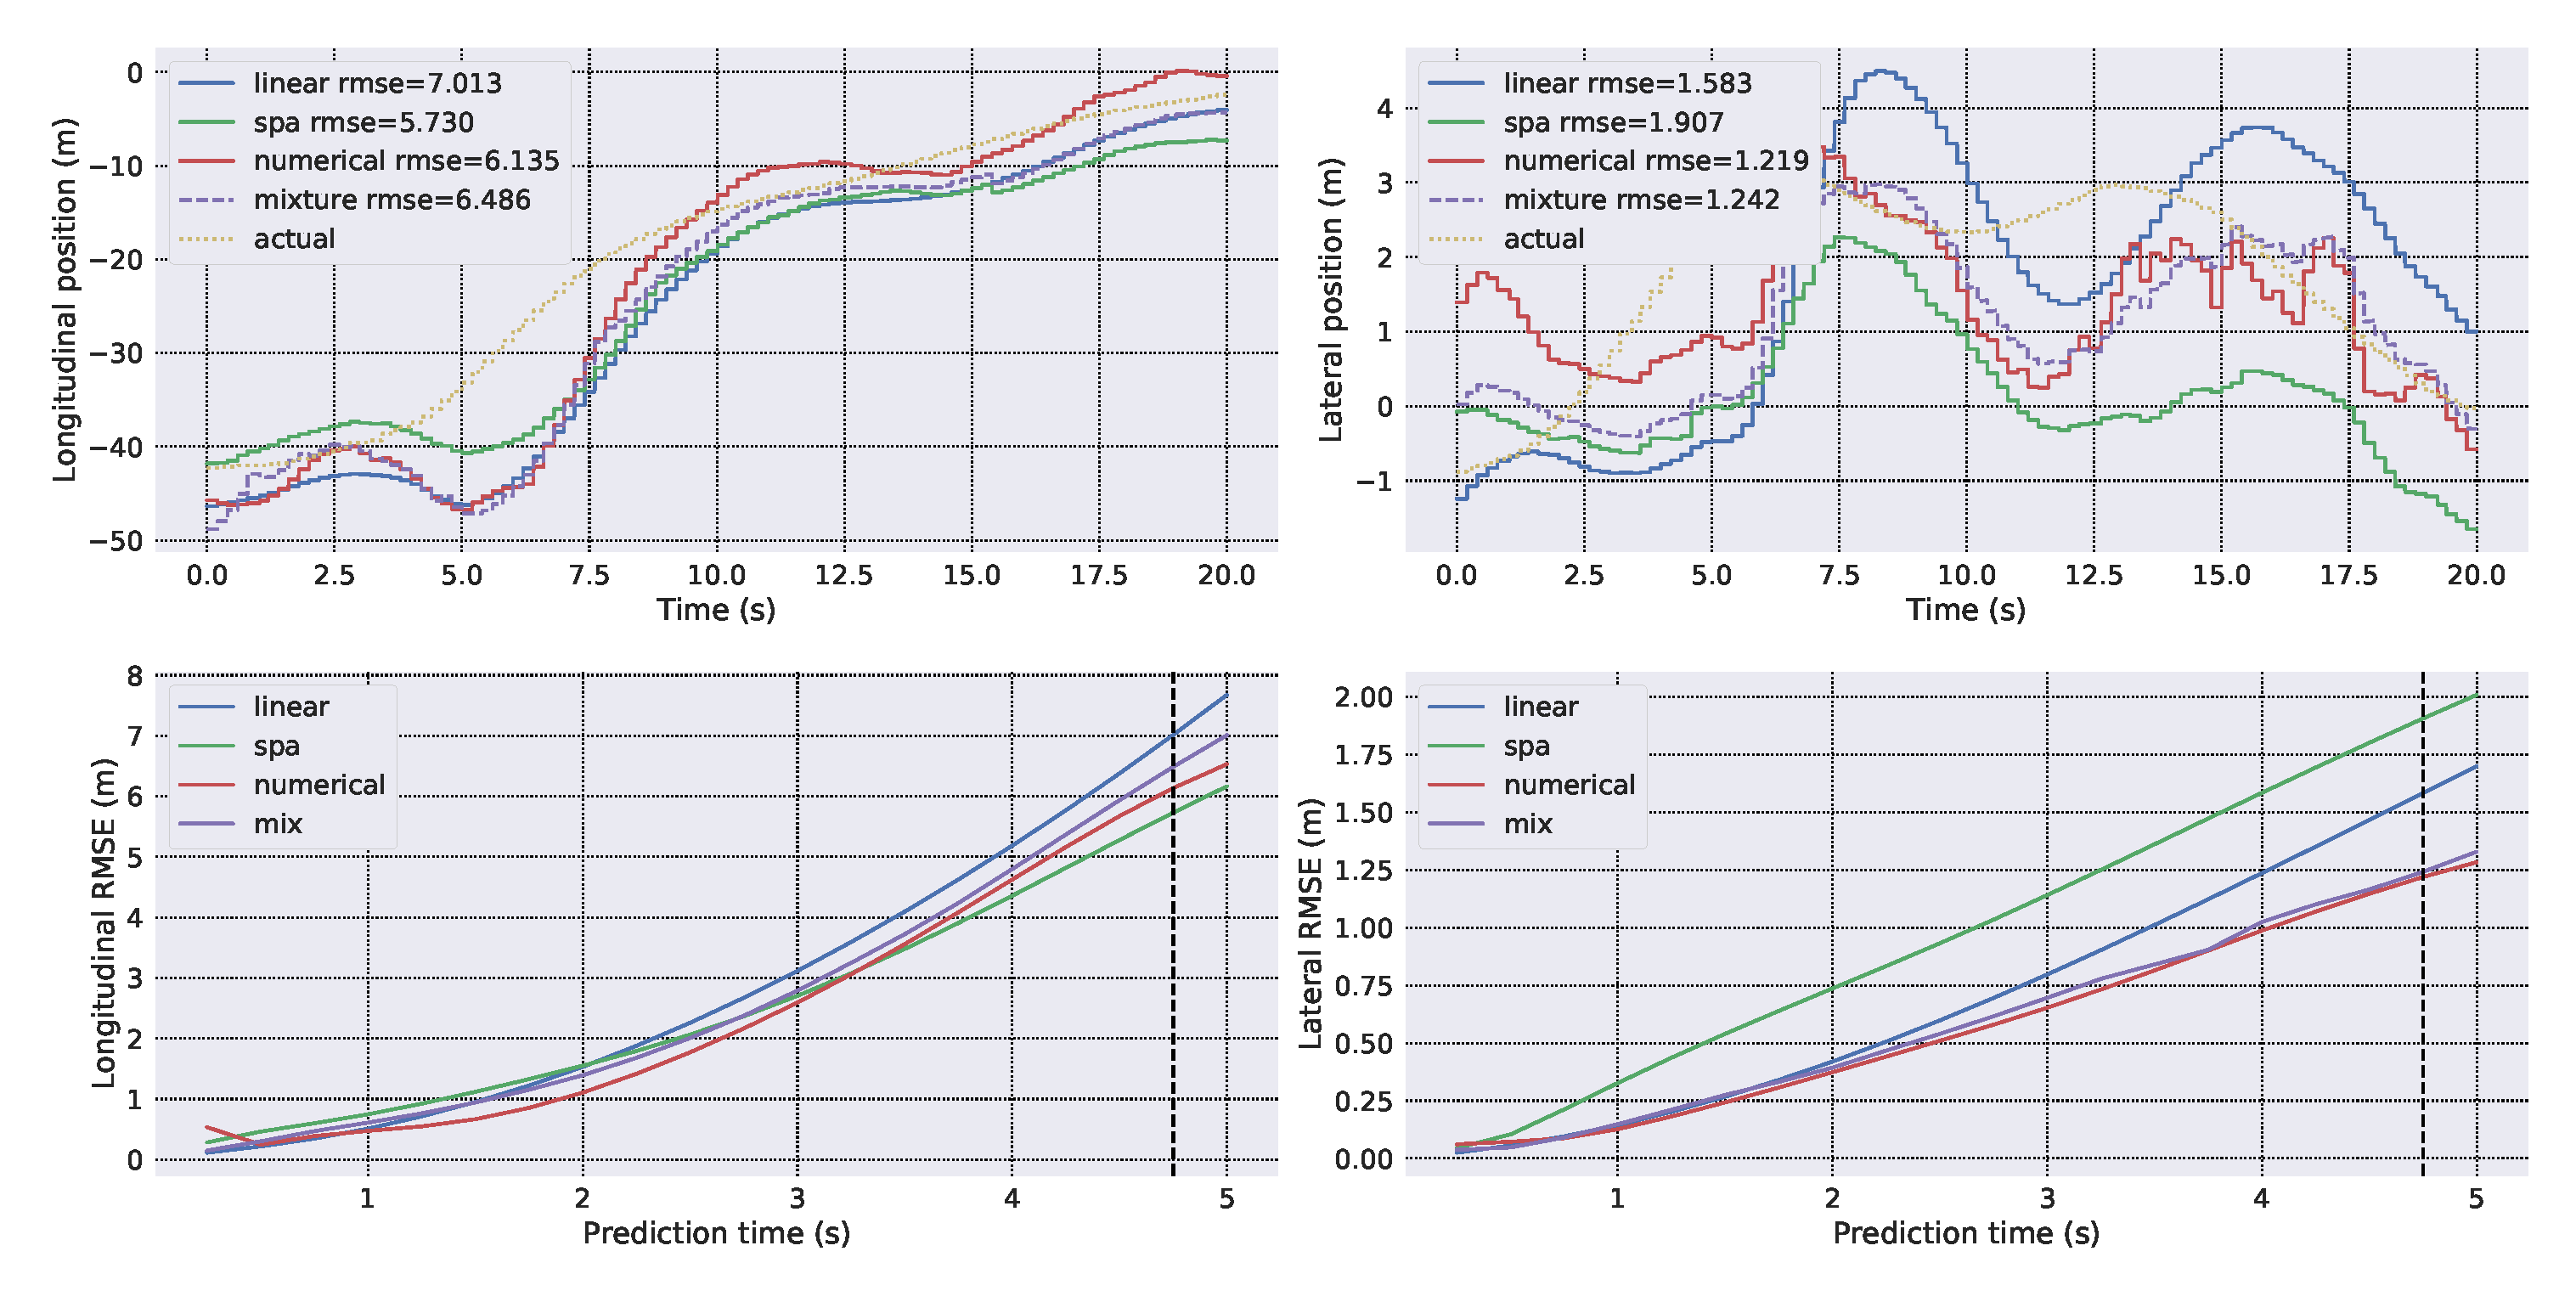
\includegraphics[width=0.8\linewidth]{imgs/mix_train_0_18.eps}
    }
    \vspace{-0.5cm}
    \subfloat[\label{subfig:mix_train_4_18}Predictions for fifth training vehicle \SI{4.75}{\second} into the future]{%
        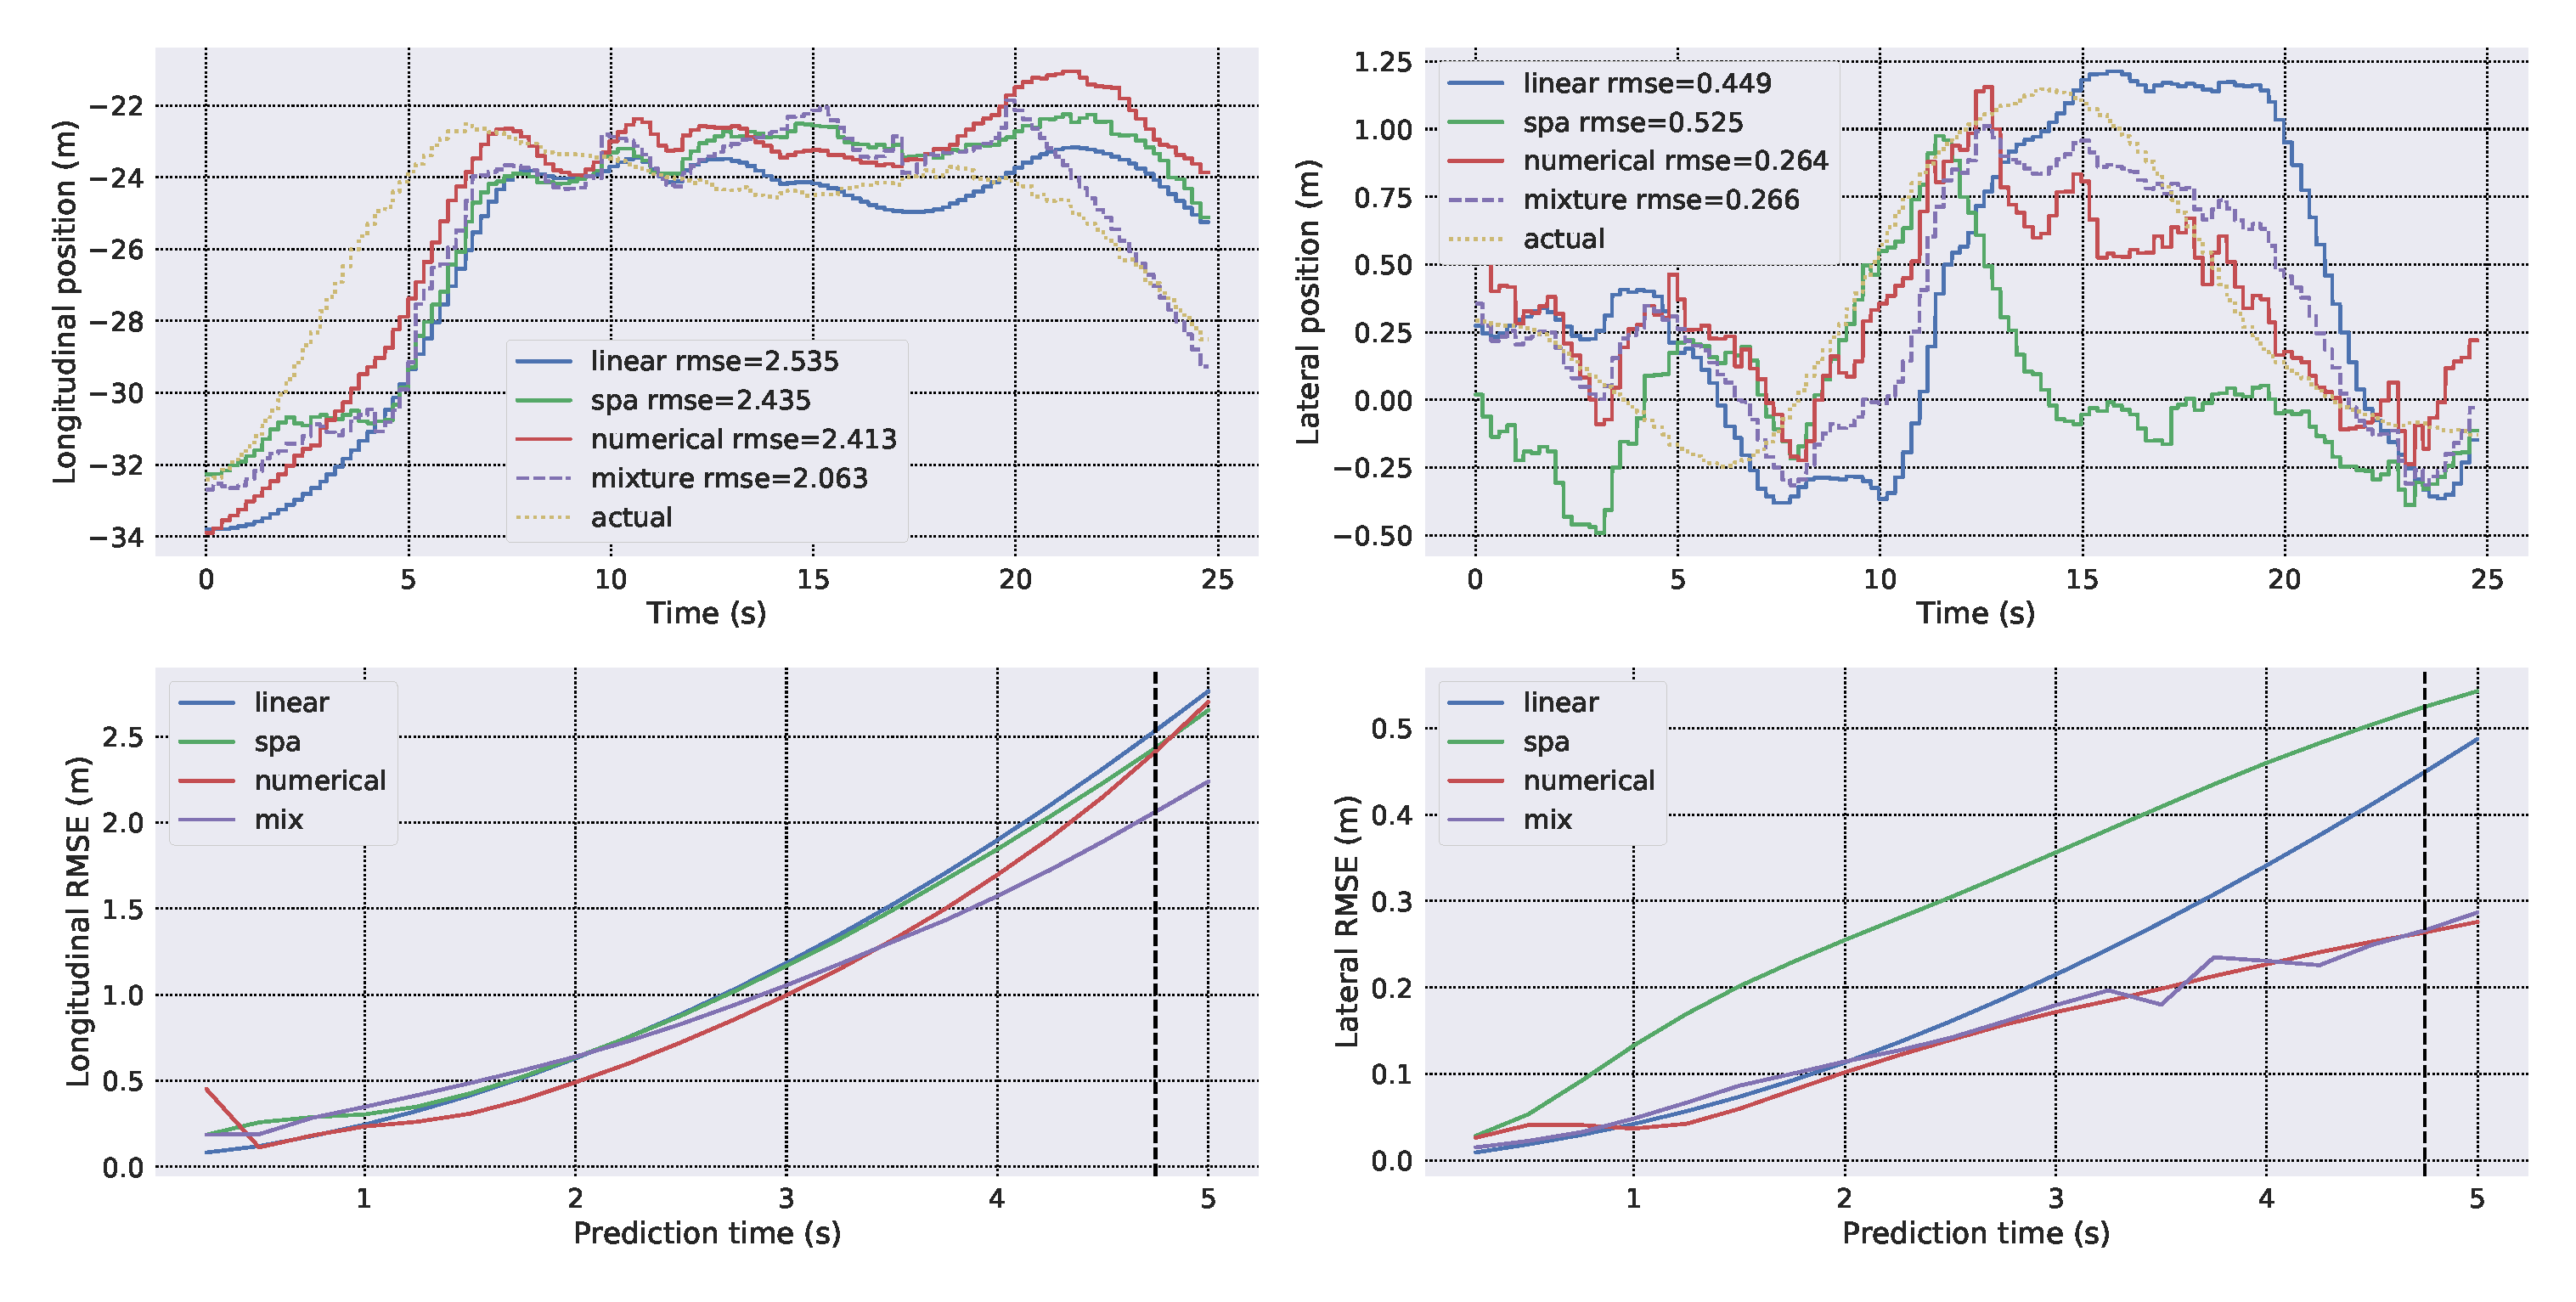
\includegraphics[width=0.8\linewidth]{imgs/mix_train_4_18.eps}
    }
    \caption{Visualization of the mixture-of-experts model's performance on vehicles it is presented during the ramp up phase.
    The upper row in each plot shows the predictions of all input predictors, the mixture model as well as the actual motion of the target vehicle for one particular prediction time step.
The lower row illustrates the \ac{RMSE} of the models on all prediction time steps with that step shown in the upper row highlighted by a dotted vertical line.}
\label{fig:mix_train_obj}
\end{figure}

Working with prerecorded data allows us to easily evaluate this simplified model before switching to the more complex version employing temporal spreading of the error signal (cf.~\ref{subsec:temporal_spreading_of_the_error_signal}).
The context-free version updates its weights solely based on the prediction error, i.e., the error between the anticipation values predicted by the model and the actual motion of the target vehicle.
This context-free approach is equivalent to the context-sensitive model if its context is kept constant.
The context-sensitive model variant as described in section~\ref{subsec:a_context_free_mixture_of_experts_online_learning_model}, which we investigate here, contains \num{3000} neurons in the population encoding the driving context.
To limit the simulation time, we exposed only a subset of \num{70} vehicles from the \emph{On-board} test set $V_1$ and \num{92} vehicles from \emph{\ac{NGSIM}} the test set $V_2$ to the models.

\subsubsection{Results}%
\label{ssubsec:results}

Figure~\ref{fig:mix_timing_agnostic} shows the results of the simplified, timing-agnostic variants of the context-free and context-sensitive mixture-of-experts online learning models on both data sets. 
Figure~\ref{subfig:mix_start_on_board} and~\ref{subfig:mix_on_board} show the models' performance on the \emph{On-board} data set at the start of training (\ref{subfig:mix_start_on_board}) and for the complete set of \num{70} evaluation vehicles from $V_1$ (\ref{subfig:mix_on_board}), whereas figure~\ref{subfig:mix_start_ngsim} and~\ref{subfig:mix_ngsim} similarly depict the models' performance on the \emph{\ac{NGSIM}} data set at the start of training and for all \num{92} evaluation
vehicles respectively.
We observe in figure~\ref{subfig:mix_start_on_board} and~\ref{subfig:mix_start_ngsim} that both, the context-free and context-sensitive mixture models perform poorly at the start of training (which makes sense due to the randomly initialized weights), but improve significantly and consistently on both data sets (figure~\ref{subfig:mix_on_board} and~\ref{subfig:mix_ngsim}) the more data they receive.
The context-free version yields mild improvements over all individual predictors in $x$-direction without improving over the best individual model in $y$-direction.
The context-sensitive variant outperforms all other models (including the context-free version) in $x$-direction while being on par with the best individual predictors in $y$-direction.

\subsection{Evaluation of the context-sensitive model variant with temporal spreading}%
\label{subsec:evaluation_of_the_context_sensitive_model_variant_with_temporal_spreading}

Having seen that the simplified mixture model using contextual information clearly outperformed the context-free version, we now proceed to the evaluation of the context-sensitive mixture-of-experts model variant having to deal with temporally delayed error signals employing our temporal spreading approach.
We describe the experimental setup, analyze several adjustable parameters of the model and finally evaluate the performance of the model given the chosen parameter setup.

\subsubsection{Experimental setup}%
\label{ssubsec:experimental_setup}

\begin{figure}[t]
    \centering
    \subfloat[\label{subfig:mix_learning_rates_even_scale_50n}\ac{RMSE} performance for varying learning rates for a fixed number of \num{50} neurons in the context population]{%
        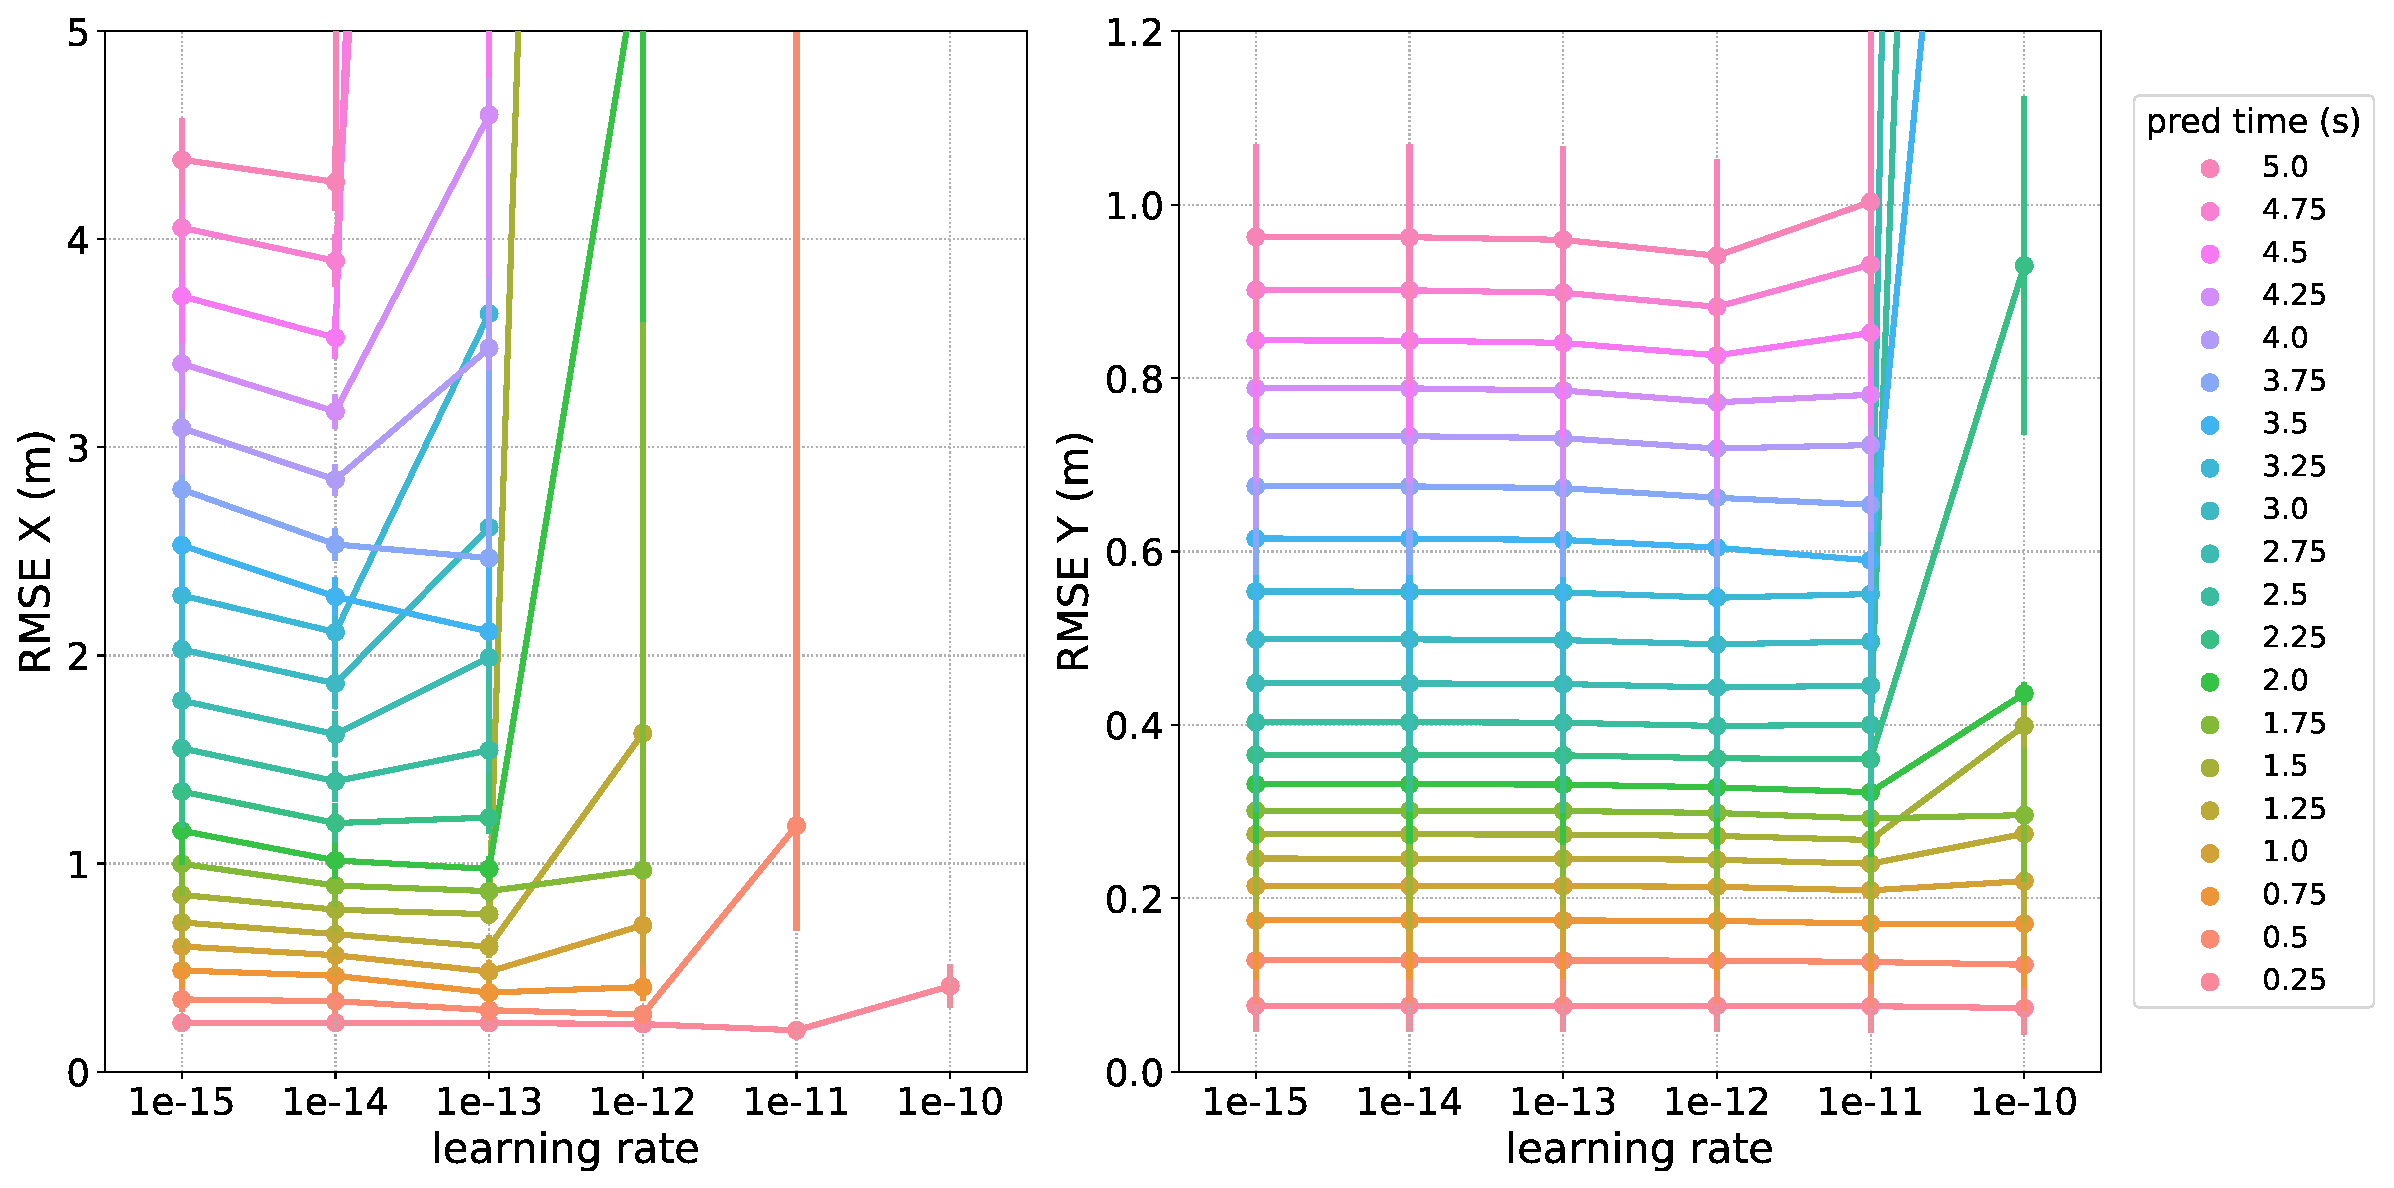
\includegraphics[width=0.8\linewidth]{imgs/mix_learning_rates_even_scale_50n.eps}
    }\\
    \subfloat[\label{subfig:mix_fail} Results of an experiment with too low of a learning rate for the mixture models resulting in high errors]{%
        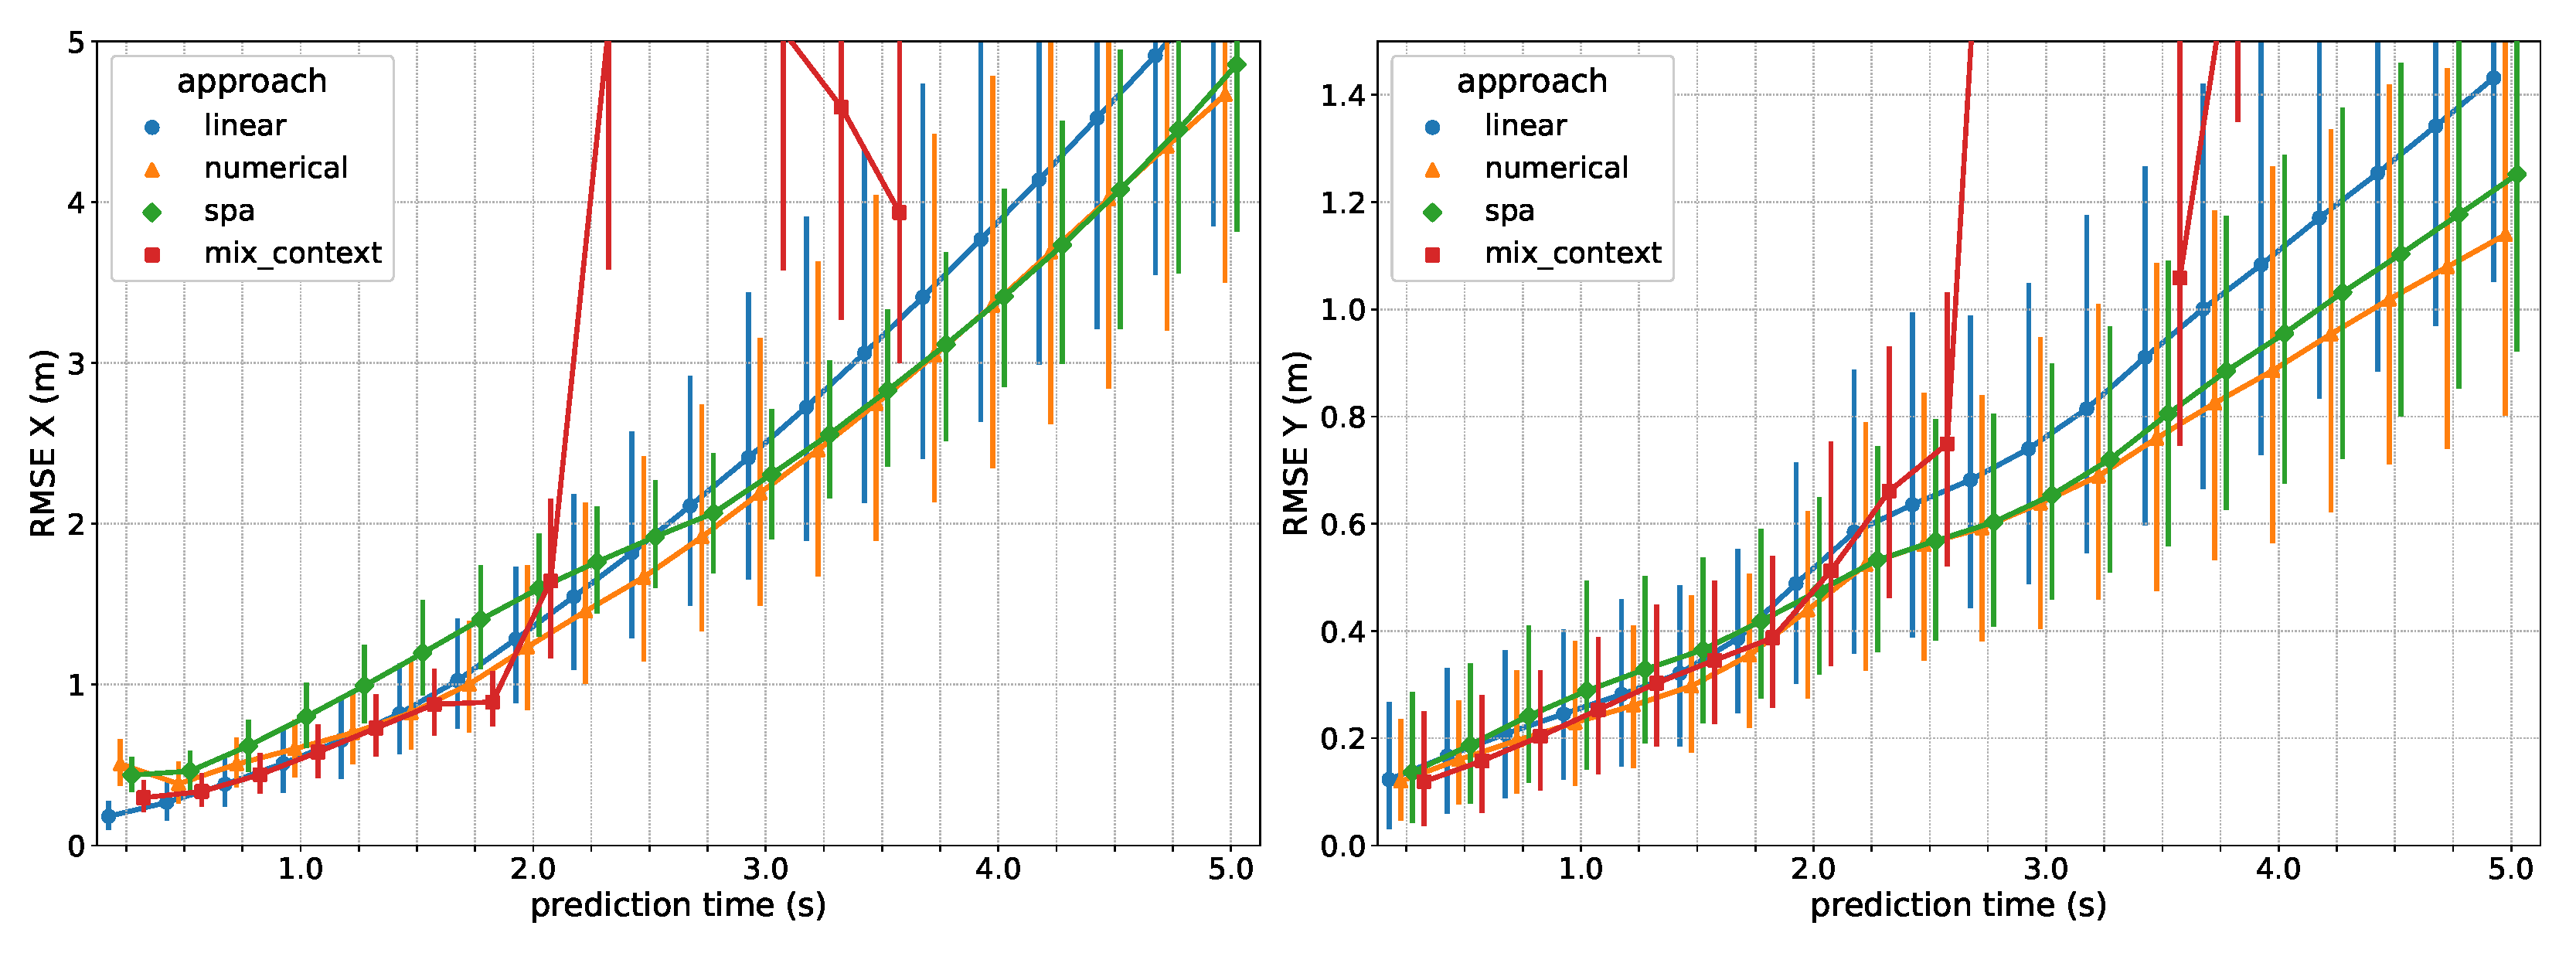
\includegraphics[width=0.8\linewidth]{imgs/mix_fail.eps}
    }
    \caption{Visualization of the \ac{RMSE} performance of our context-sensitive mixture-of-experts model using temporal spreading on \num{30} test vehicles after being trained on \num{5} vehicles for~\protect\subref{subfig:mix_learning_rates_even_scale_50n} different learning rates for all prediction horizons and~\protect\subref{subfig:mix_fail} the result of one evaluation run with too low of a learning rate.}
    \label{fig:mix_parameters1}
\end{figure}

To evaluate feasibility and performance of our mixture-of-experts model having to deal with temporally delayed error signals, we conducted our experiments for both, the parameter analysis as well as the actual performance evaluation, in the following way:
after randomly initializing the weights of the mixture model, we present the data of \num{5} randomly chosen vehicles to the model to make sure the weights depart reasonably from their initial values.
After this ramp-up phase, during which we conduct no evaluation, the model is presented with \num{30} more randomly chosen vehicles to be evaluated on.
During the presentation of these \num{30} test vehicles, the mixture model continues to adapt its weights depending on the current error and context.

Figure~\ref{fig:mix_train_obj} shows the performance of the mixture model with \num{50} neurons in the context population for selected vehicles during the \num{5}-vehicle ramp up phase.
The upper row in each plot shows the predictions of all input predictors, the mixture model as well as the actual motion of the target vehicle for one particular prediction time step.
For instance, the upper row in figure~\ref{subfig:mix_train_0_2} illustrates the predictions of all models for \SI{0.75}{\second} into the future over the complete time the target vehicle is visible.
The lower row in each plot illustrates the \ac{RMSE} of the models for all prediction time steps with the particular time step shown in the upper row highlighted by a dotted vertical line.
Figures~\ref{subfig:mix_train_0_2} and~\ref{subfig:mix_train_0_18} show the prediction time steps \SIlist{0.75;4.75}{\second} into the future respectively of the first vehicle during the ramp-up phase while figure~\ref{subfig:mix_train_4_18} shows the prediction time step \SI{4.75}{\second} into the future for the last vehicle of the ramp-up phase.
We observe, that the even distributed weights are a reasonable initialization for further adaptation by our model , since already for the first vehicle presented to the model achieves a decent prediction accuracy.
Reaching the fifth training vehicle, the mixture model already achieves improvements for prediction time-steps further into the future in $x$-direction and equal to the best performing input predictor.

\subsubsection{Parameter analysis}%
\label{ssubsec:parameter_analysis}

\begin{figure}[t]
    \centering
    \subfloat[\label{subfig:mix_learning_rate_analysis}\ac{RMSE} performance for varying learning rates for a fixed number of \num{100} neurons in the context population]{%
        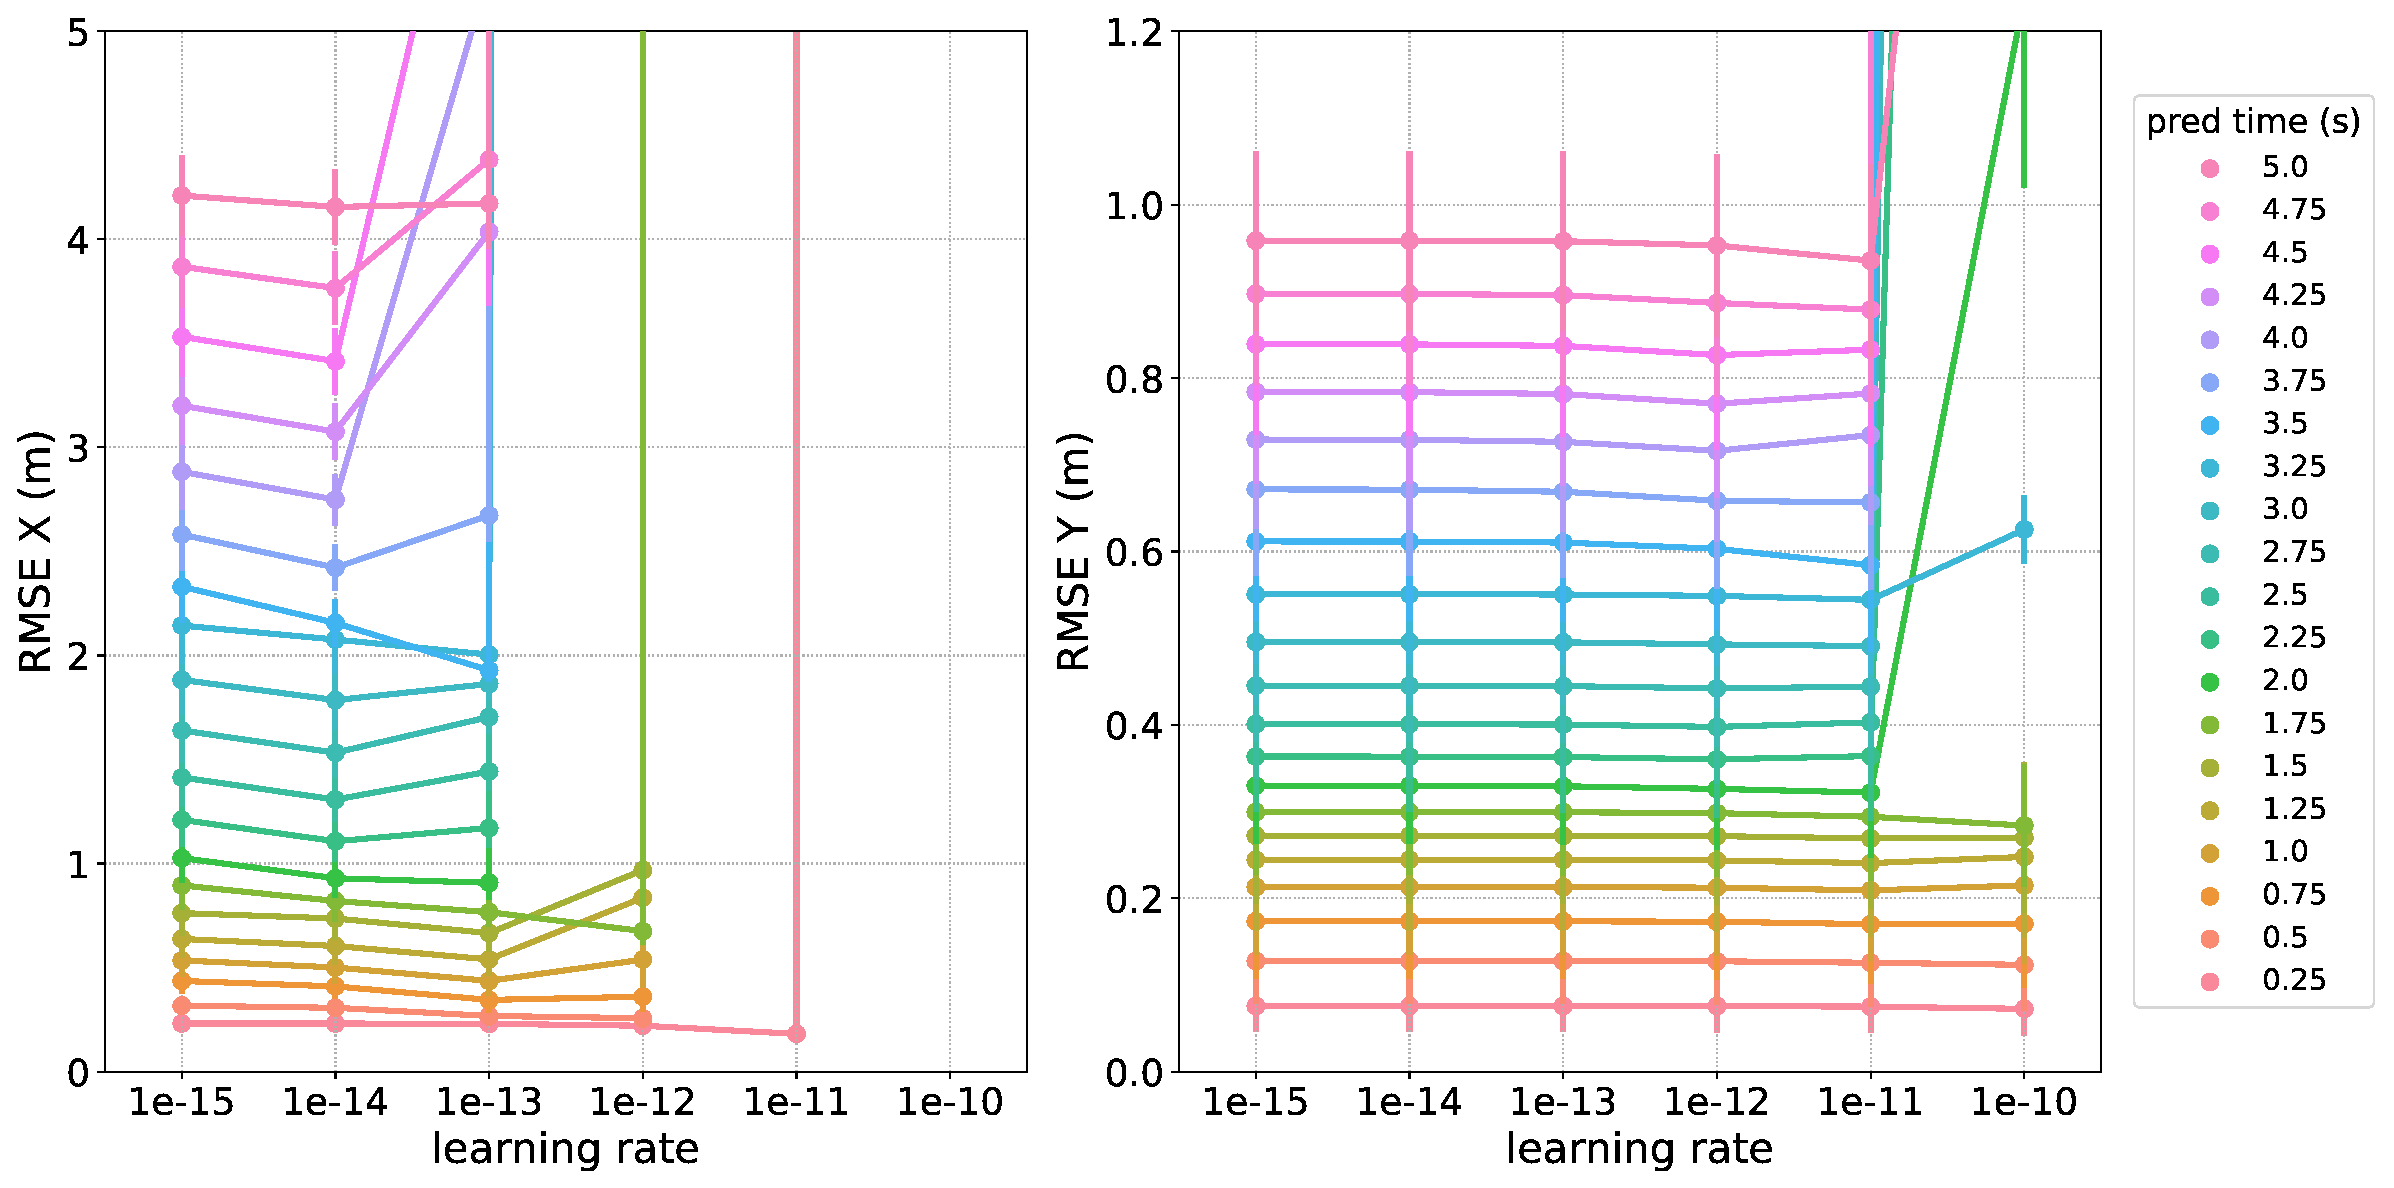
\includegraphics[width=0.8\linewidth]{imgs/mix_learning_rate_analysis.eps}
    }\\
    \subfloat[\label{subfig:mix_num_neuron_analysis}\ac{RMSE} performance for varying number of neurons in the context population for a fixed learning rate of \num{e-15}]{%
        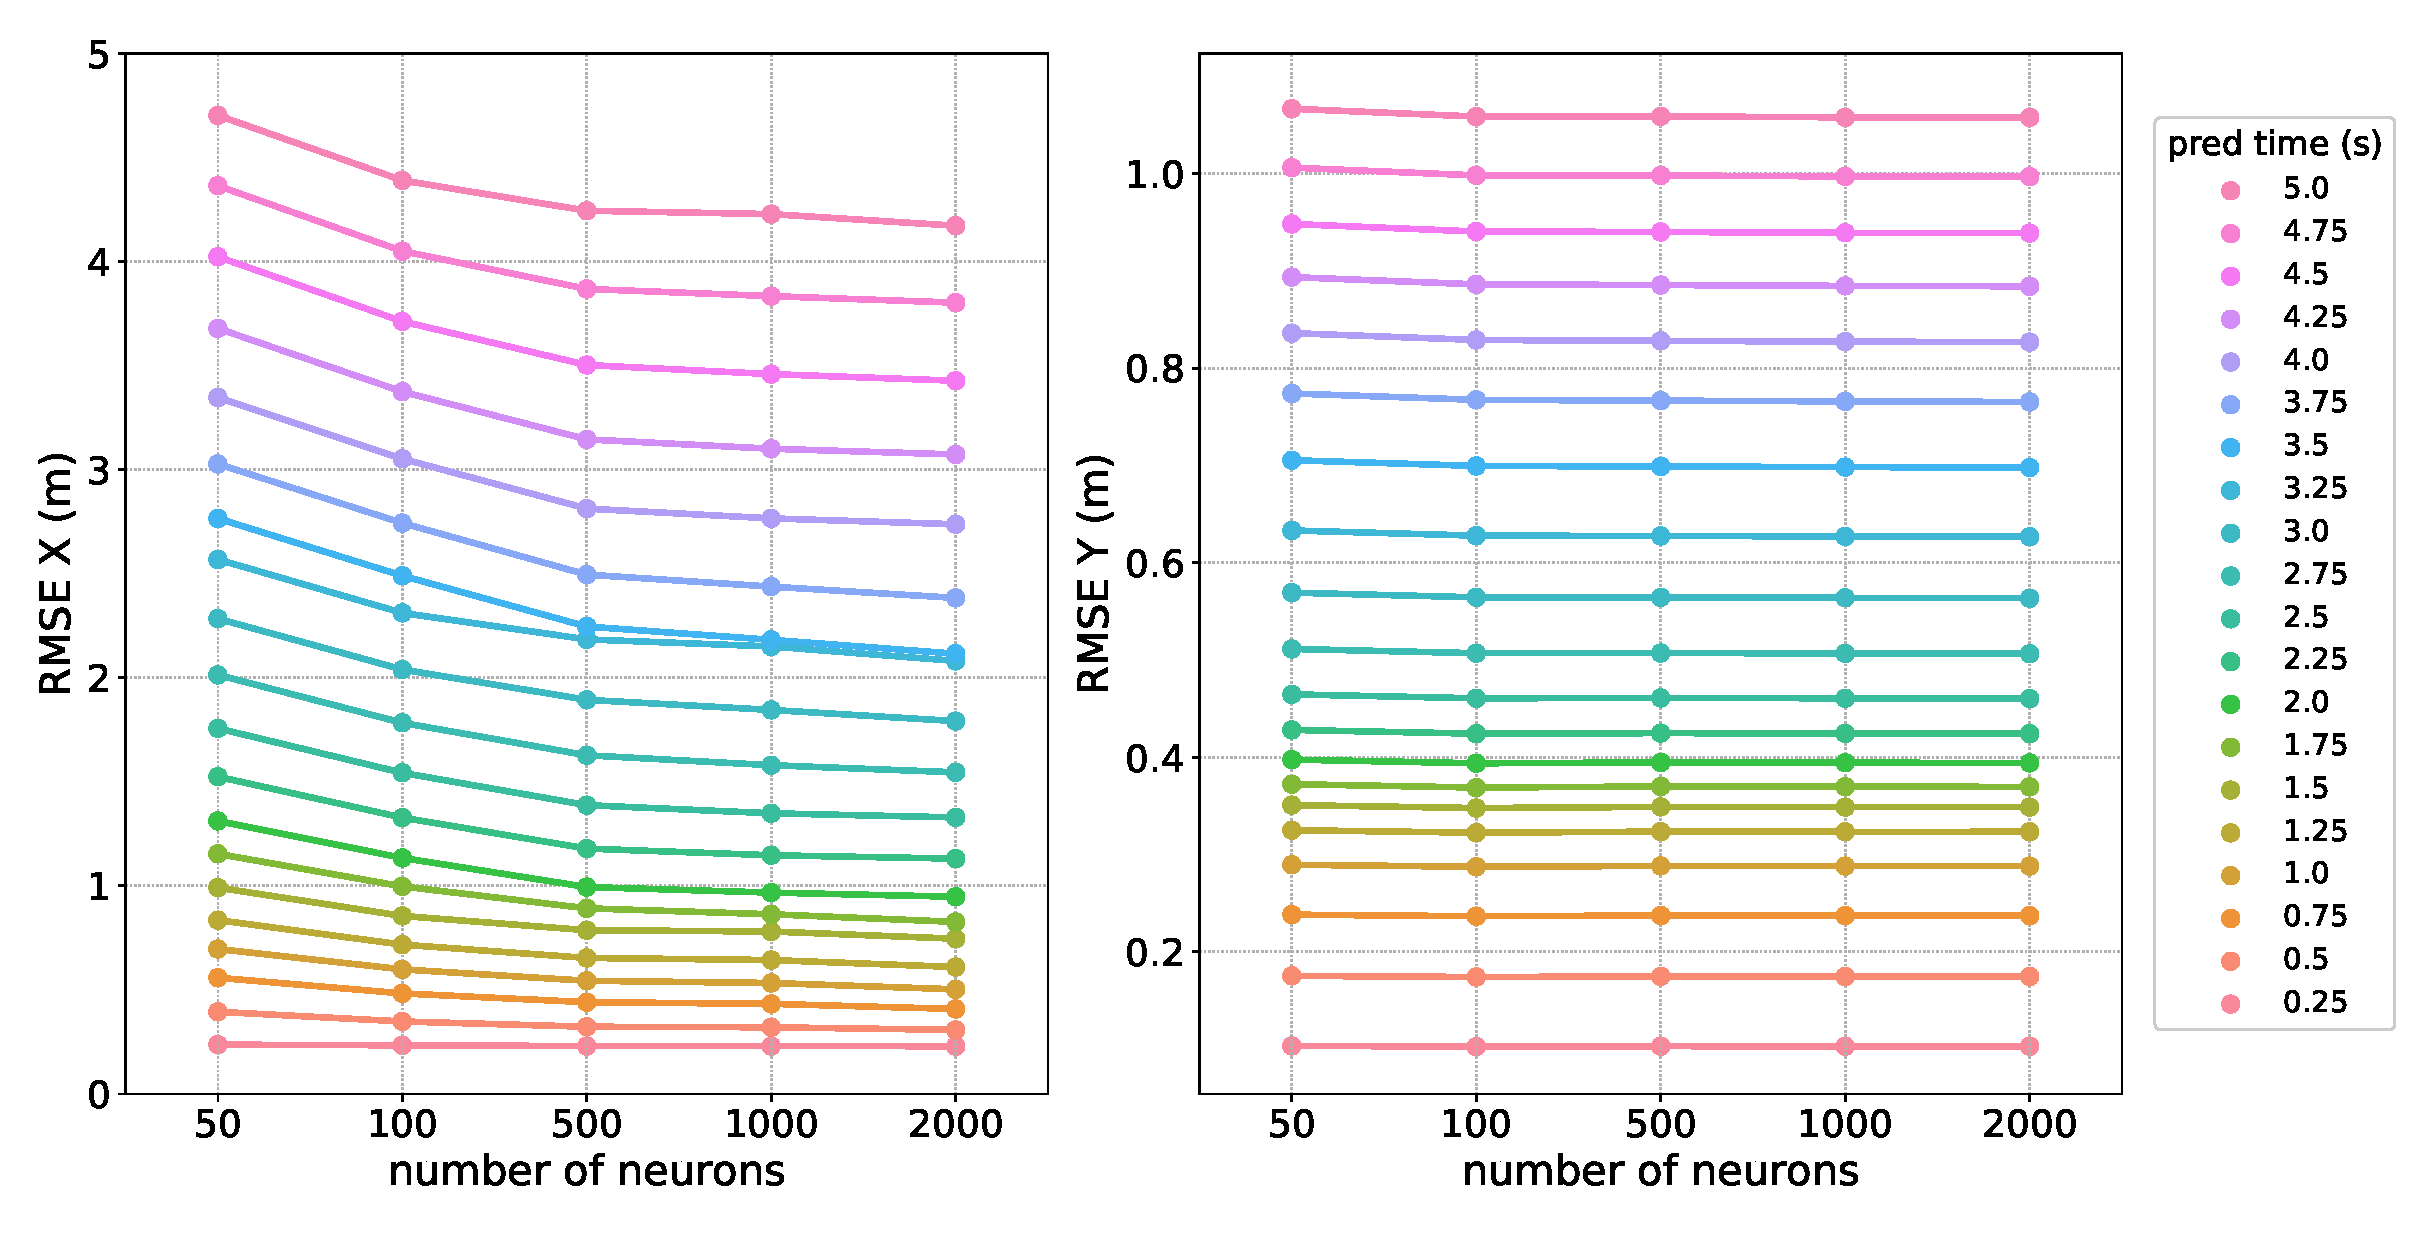
\includegraphics[width=0.8\linewidth]{imgs/mix_num_neuron_analysis.eps}
    }
    \caption{Visualization of the \ac{RMSE} performance of our context-sensitive mixture-of-experts model using temporal spreading on \num{30} test vehicles after being trained on \num{5} vehicles for certain hyper-parameter variations.}
    \label{fig:mix_parameters2}
\end{figure}

To find the best possible variant of our mixture-of-experts model, we first analyzed the adjustable parameters of the model. 
Figure~\ref{fig:mix_parameters1} shows a visualization of the \ac{RMSE} performance of our context-sensitive mixture-of-experts model using temporal spreading on \num{30} test vehicles after being trained on \num{5} vehicles.
Figure~\ref{subfig:mix_learning_rates_even_scale_50n} visualizes the \ac{RMSE} performance of our mixture-model with \num{50} neurons in the context population for different values of the learning rate $\kappa$ with scaling factors $\nu_{t}=1$ for all prediction time steps $t$.
In this evaluation, a learning rate of $10^{-14}$ in $x$-direction and $10^{-12}$ show the best performance.
However, figure~\ref{subfig:mix_fail} shows the results of a model variant with \num{2000} neurons in the context population employing these learning rates for a different set of vehicles.
We observe, that the model performs well for earlier prediction horizons but fails to make accurate prediction further into the future with very high errors and even complete failure due to overfitting.

Therefore, we focus on scaling factors $\nu_t$ decreasing linearly from \num{1} to \num{0.001} over the \num{20} prediction times with \num{1} corresponding to the earliest prediction step to ensure low enough learning rates prediction time steps further into the future.
Figure~\ref{fig:mix_parameters2} shows a visualization of the \ac{RMSE} performance of our mixture-model with \num{100} neurons in the context population with for different values of the learning rate $\kappa$.
Figure~\ref{subfig:mix_learning_rate_analysis} shows an analysis similar to figure~\ref{subfig:mix_learning_rates_even_scale_50n} but using the linearly decreasing scaling factors.
We observe, that the scaling the learning rates down stabilizes the model compared to the even scaling factors.
As already shown in figure~\ref{subfig:mix_fail}, we found that a rather low learning rate $\kappa$ is necessary as higher learning rates tend to let the model overfit the current vehicle, which leads to large errors and even complete failure when switching from one vehicle to the next.
We observe that issue in particular in $x$-direction when already a learning rate of $\kappa = 10^{-13}$ leads to large errors and even failure.
Given the results shown in figure~\ref{subfig:mix_fail}, we use a learning rate of $\kappa=10^{-15}$.
As the evaluation shown in figure~\ref{fig:mix_parameters2} included only \num{30} test vehicles, we chose this rather conservative learning rate to make sure our model does not overfit when using a different set of vehicles.

Furthermore, we investigated the influence of the number of neurons in the context ensemble on the model's performance employing the aforementioned values for the learning rate $\kappa$ and scaling factors $\nu_{t}$.
Figure~\ref{subfig:mix_num_neuron_analysis} shows the \ac{RMSE} of the model for varying numbers of neurons in the context population. 
In $y$-direction, the influence of the number of neurons is nearly invisible, whereas in $x$-direction increasing the number of neurons results in lower \ac{RMSE} values.
Thus, we focus our further investigations on models with \num{2000} neurons in the context population.

\subsubsection{Results of the mixture-model using temporal spreading}%
\label{ssubsec:results_of_the_mixture_model_using_temporal_spreading}

\begin{figure}[t]
    \centering
    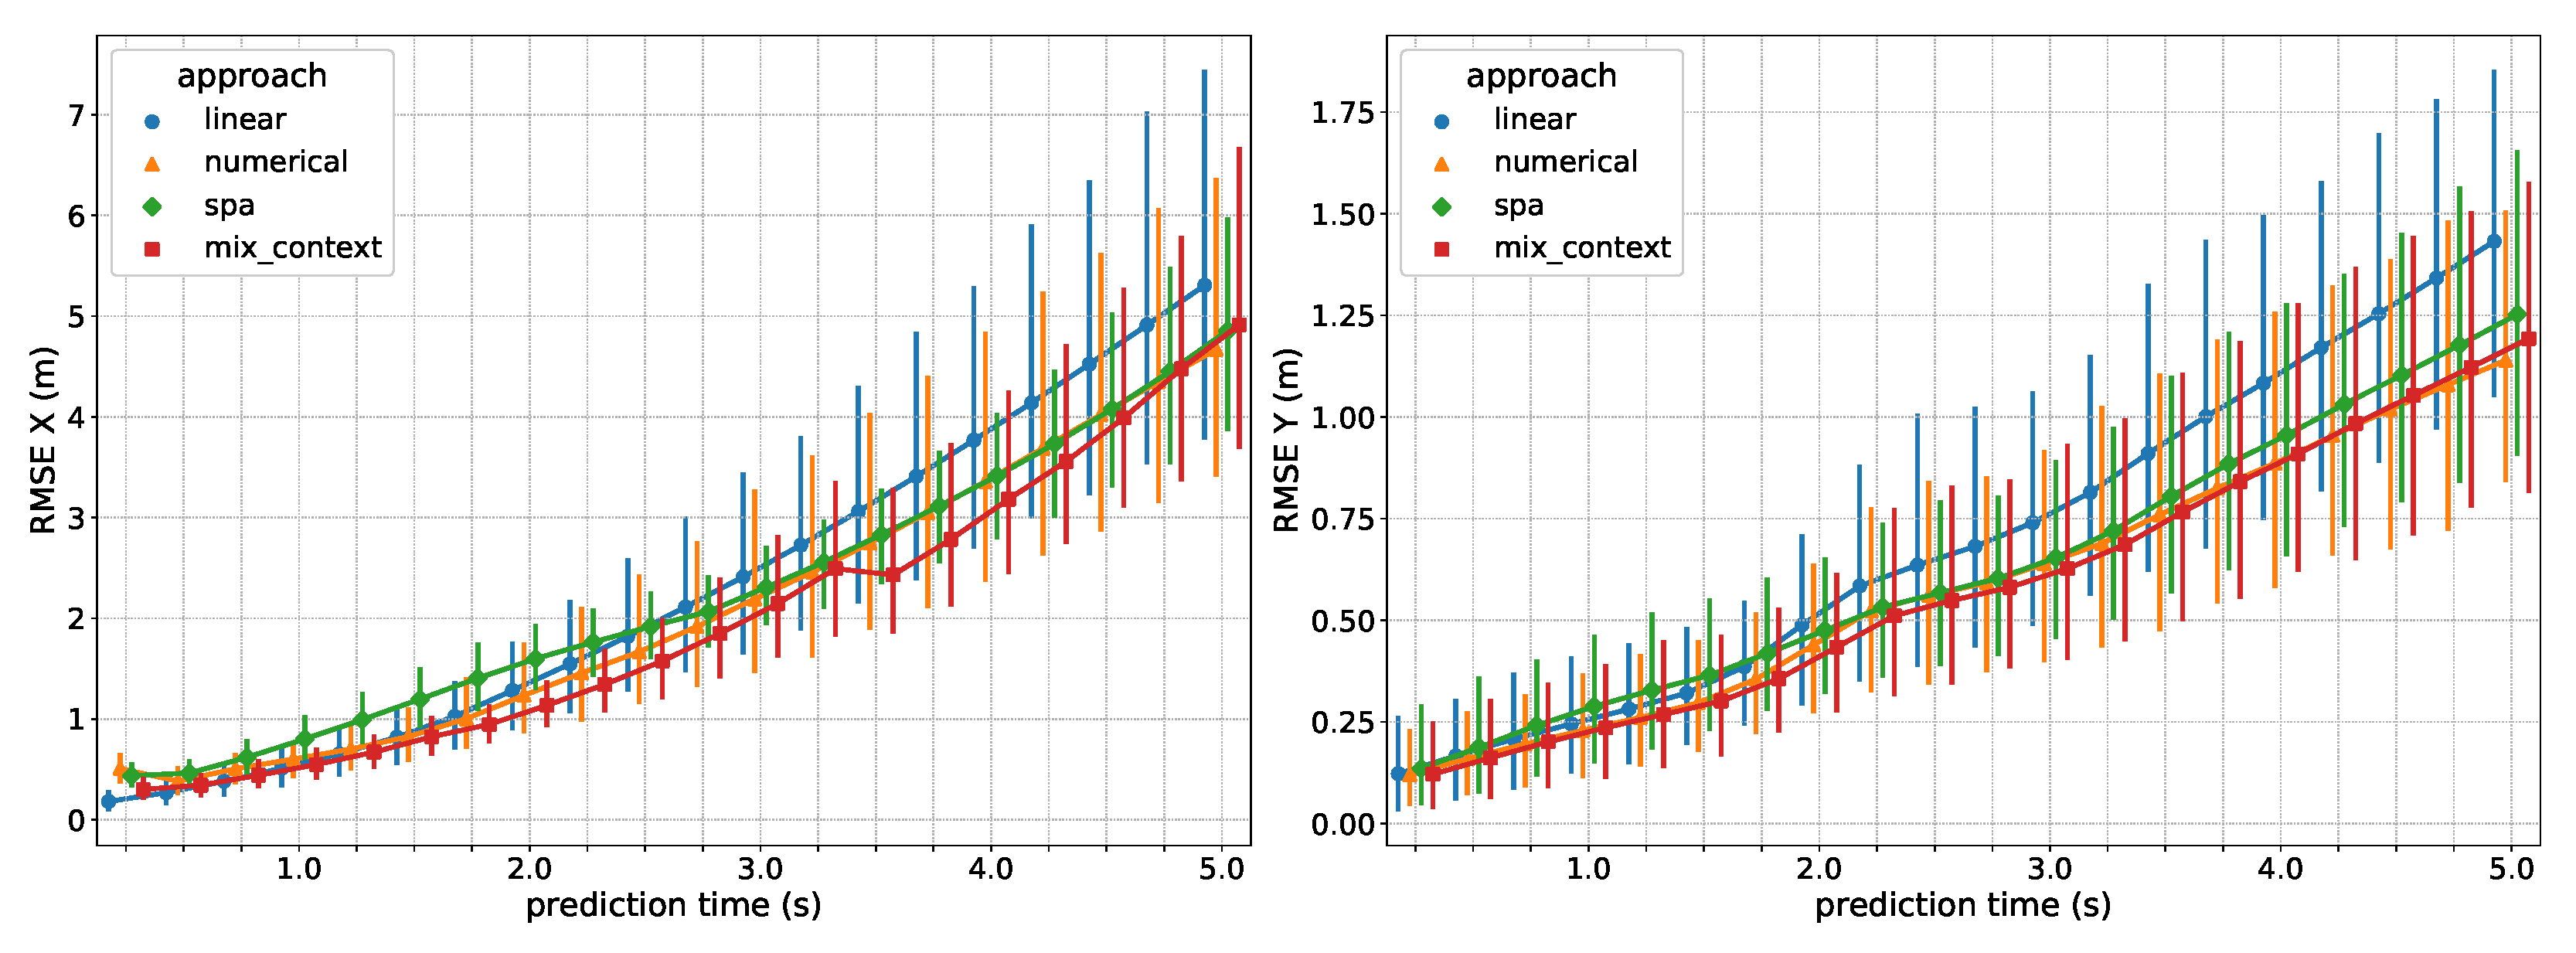
\includegraphics[width=0.95\linewidth]{imgs/mix_vs_other_approaches_over_objects.eps}
    \caption{Visualization of the \ac{RMSE} performance of all individual expert predictors as well as our context-sensitive and temporal spreading mixture-of-experts model with \num{2000} neurons in the context population, evaluated on \num{30} vehicles after the mixture model has been trained on \num{5} vehicles in advance to make the weights depart reasonably from their random initialization.}
    \label{fig:mix_vs_other_approaches_over_objects}
\end{figure}

Figure~\ref{fig:mix_vs_other_approaches_over_objects} shows the \ac{RMSE} performance of our context-sensitive mixture-of-experts model employing temporal spreading with \num{2000} neurons on the \num{30} test vehicles in comparison to the individual input predictors after the ramp-up phase of \num{5} vehicles.
We observe, that our mixture-of-experts model improves over the individual models on average over all \num{30} test vehicles in both directions without clearly outperforming them.

\begin{figure}[t]
	\centering
    \subfloat[\label{subfig:mix_vehicle_1}]{%
        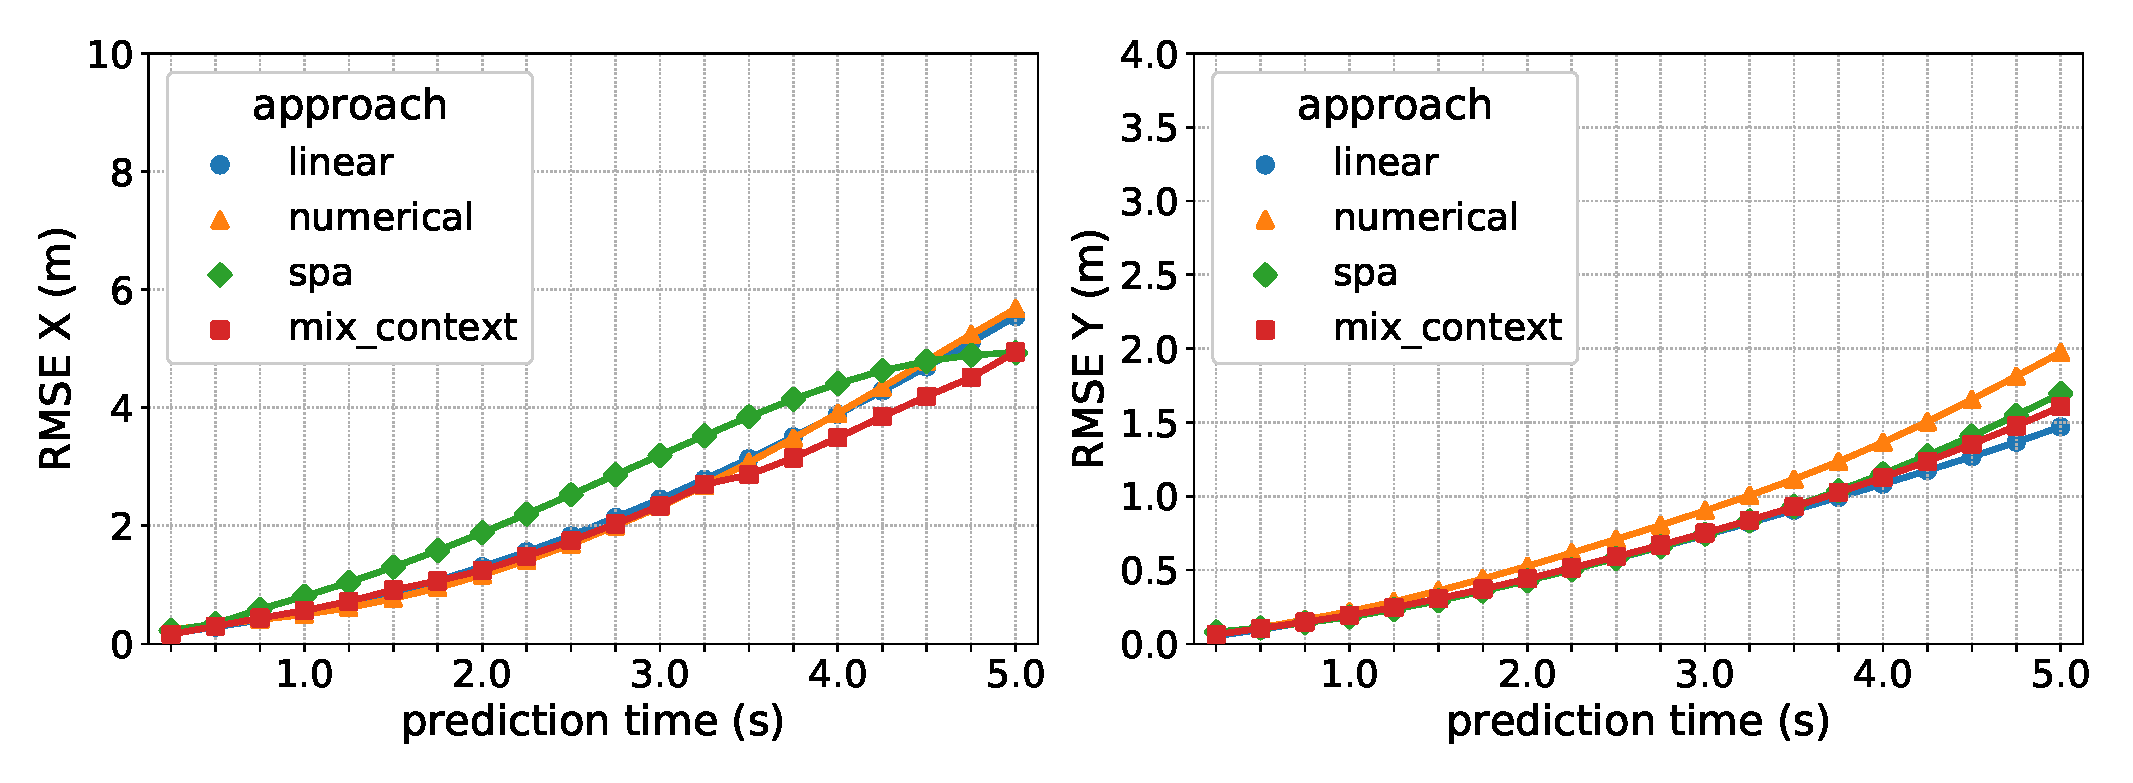
\includegraphics[width=0.5\linewidth]{imgs/mix_vehicle_1.eps}
    }
    \subfloat[\label{subfig:mix_vehicle_2}]{%
        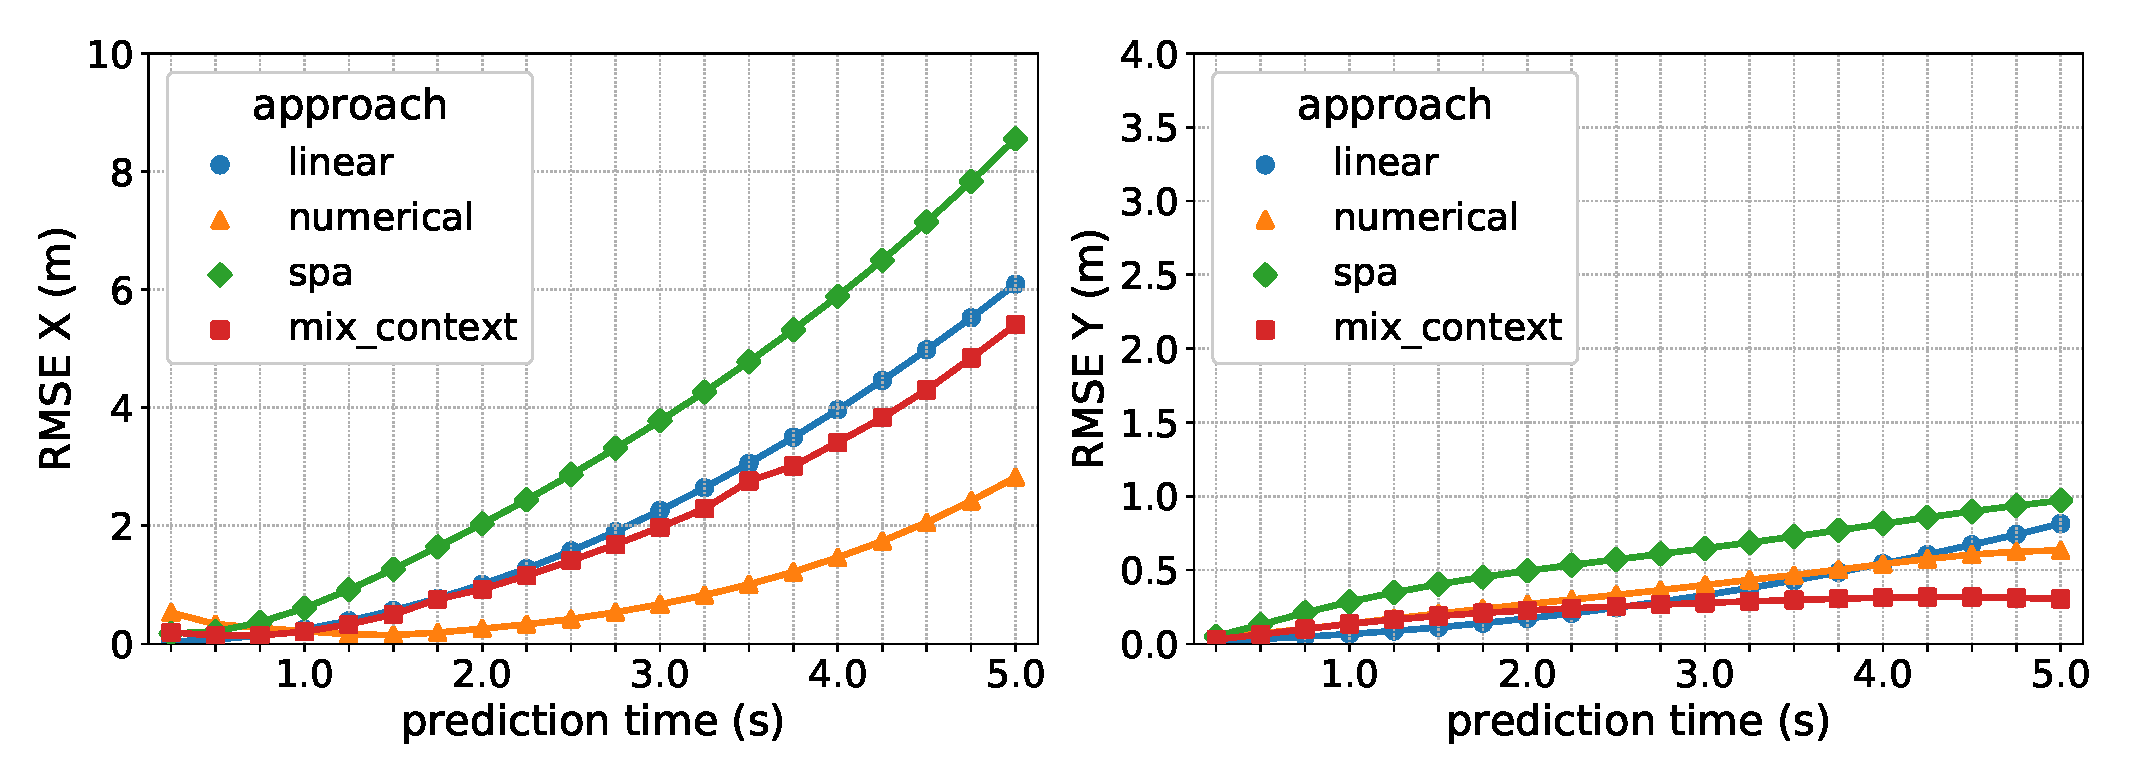
\includegraphics[width=0.5\linewidth]{imgs/mix_vehicle_2.eps}
    }
    \\
    \subfloat[\label{subfig:mix_vehicle_3}]{%
        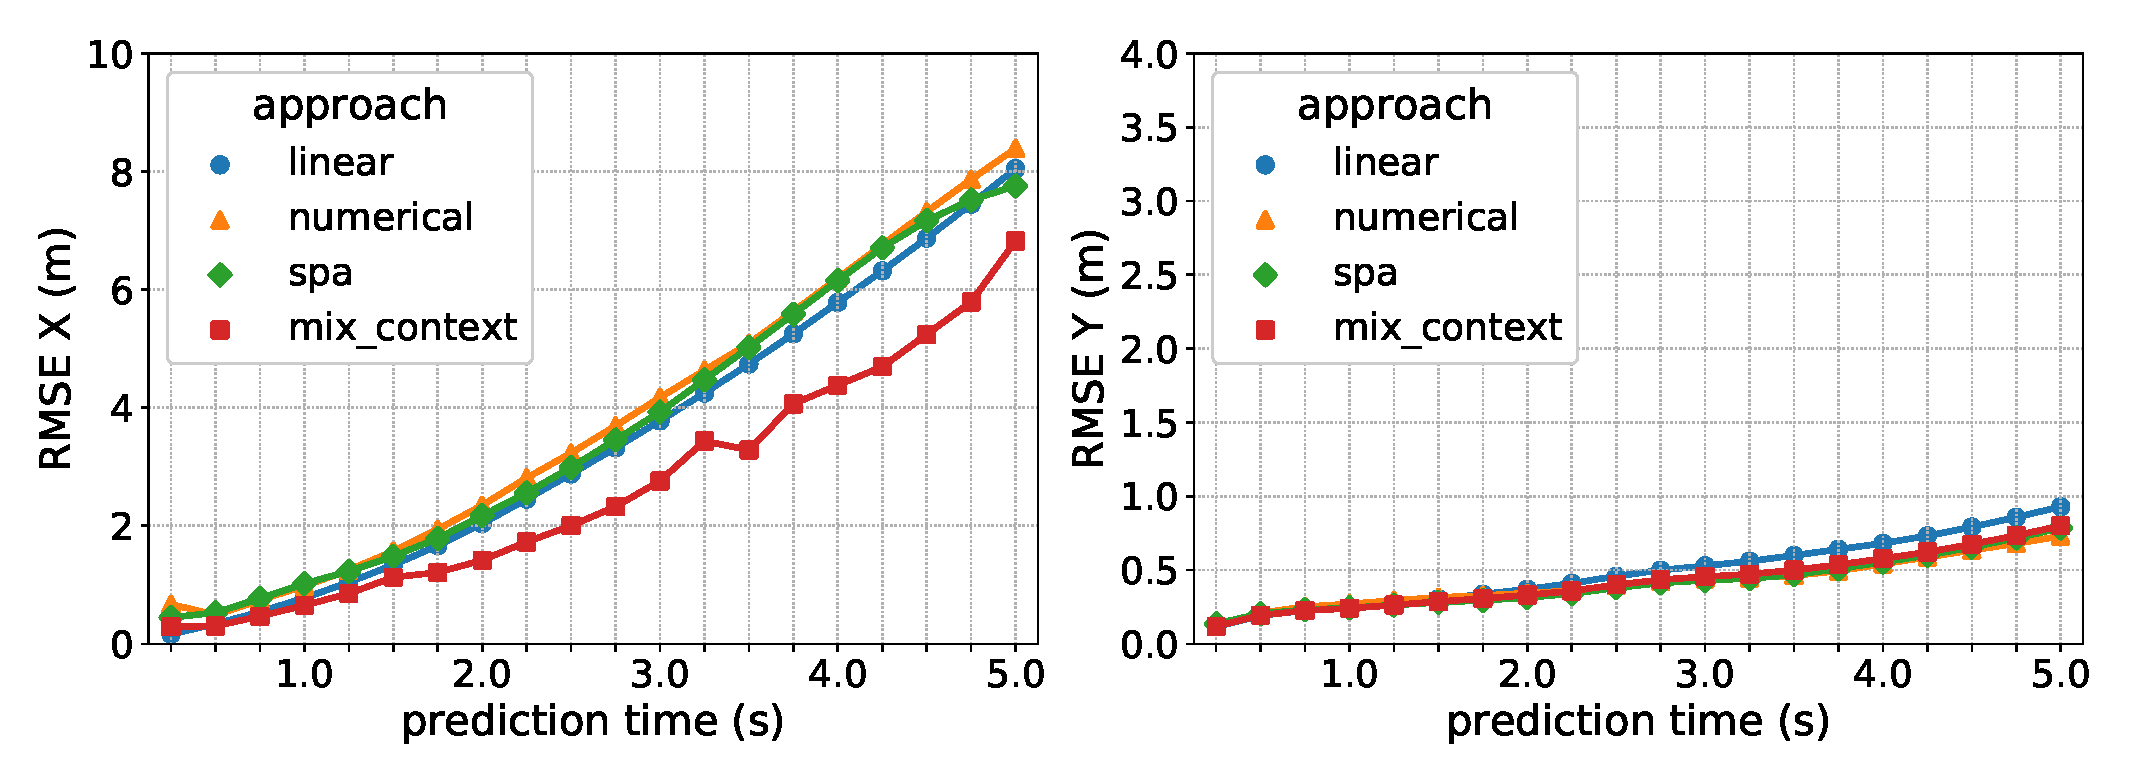
\includegraphics[width=0.5\linewidth]{imgs/mix_vehicle_3.eps}
    }
    \subfloat[\label{subfig:mix_vehicle_4}]{%
        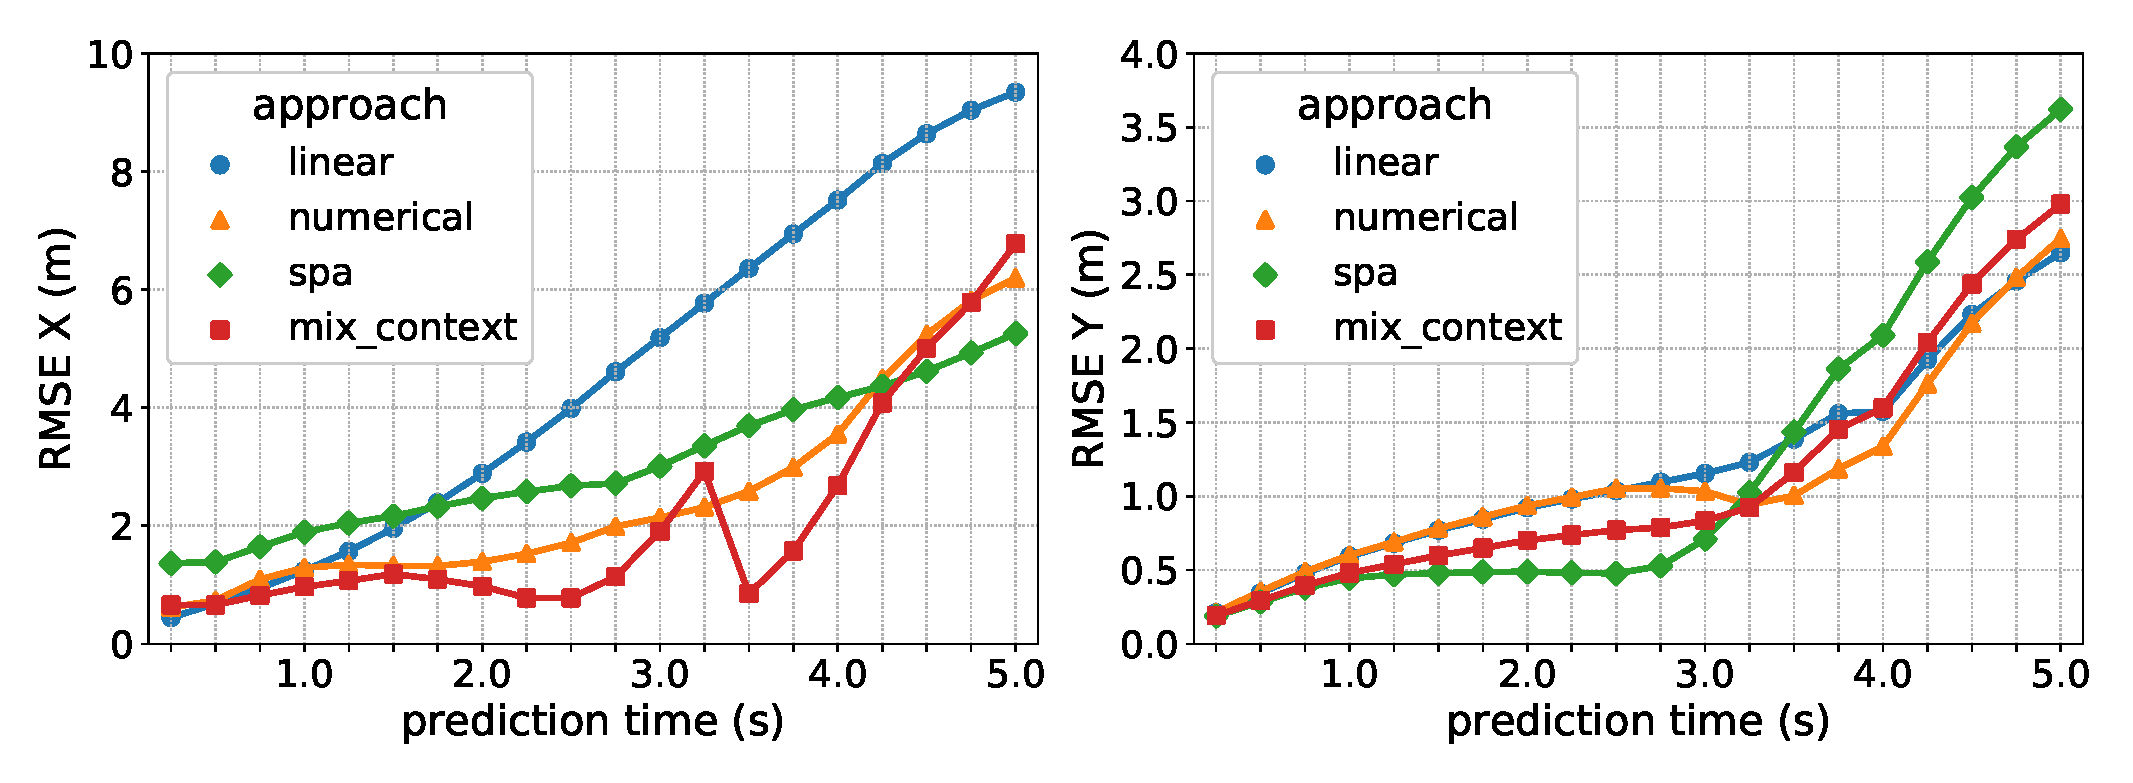
\includegraphics[width=0.5\linewidth]{imgs/mix_vehicle_4.eps}
    }
    \\
    \subfloat[\label{subfig:mix_vehicle_5}]{%
        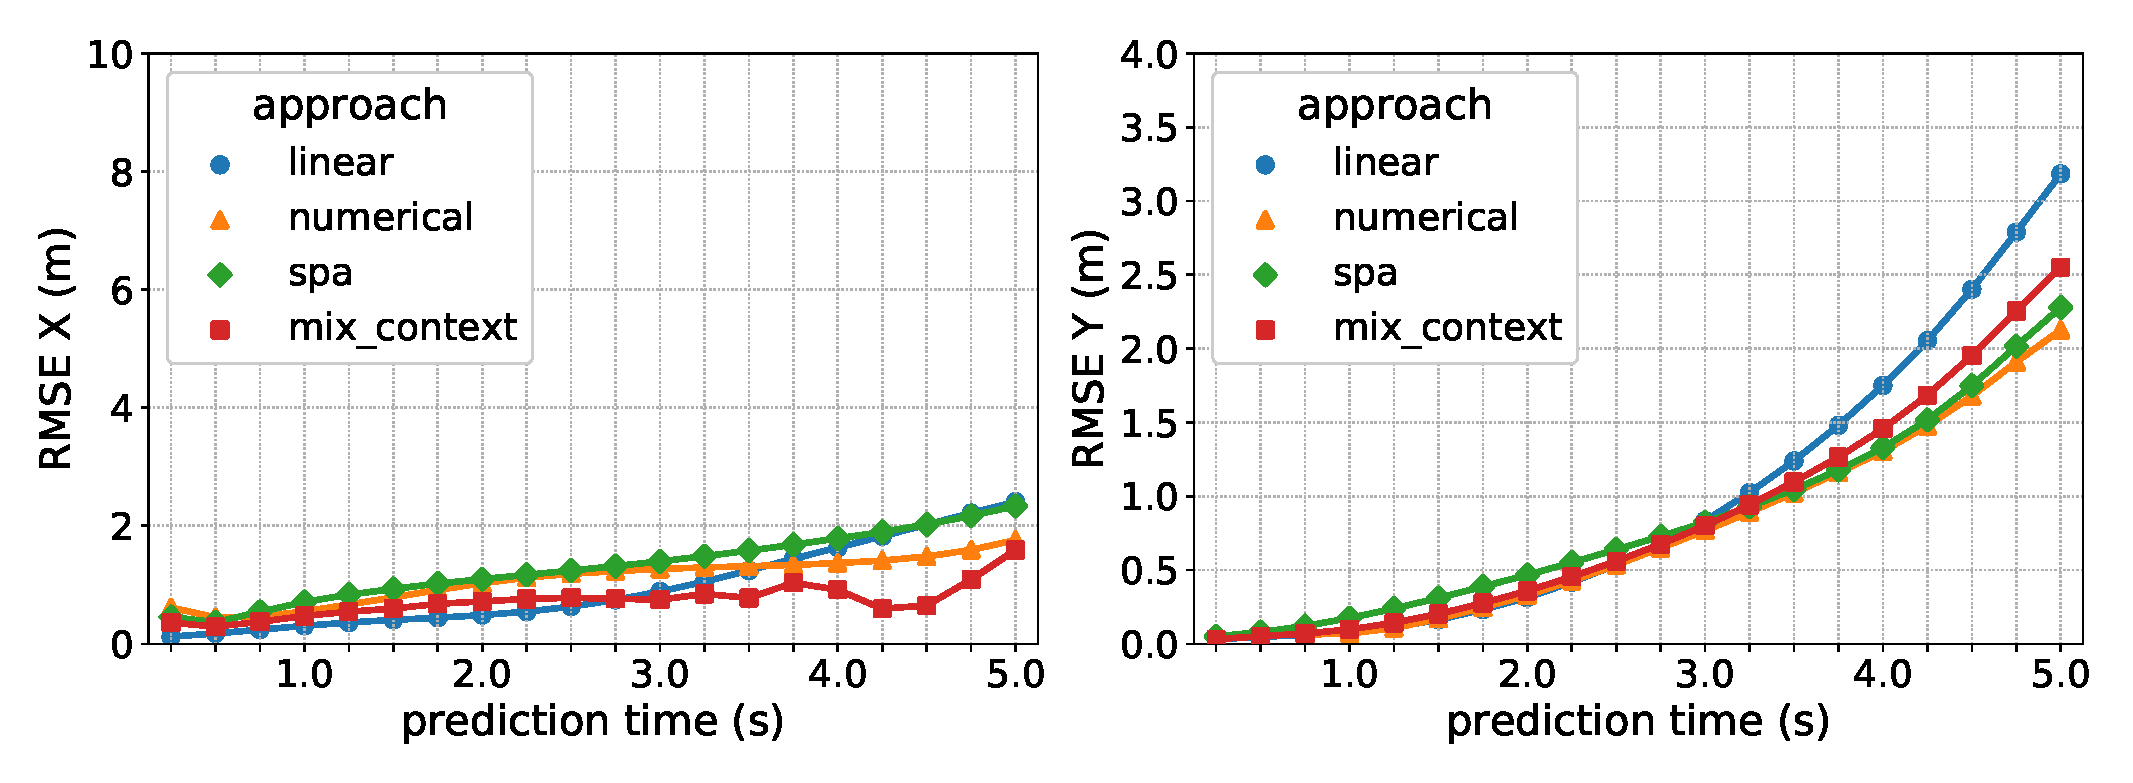
\includegraphics[width=0.5\linewidth]{imgs/mix_vehicle_5.eps}
    }
    \subfloat[\label{subfig:mix_vehicle_6}]{%
        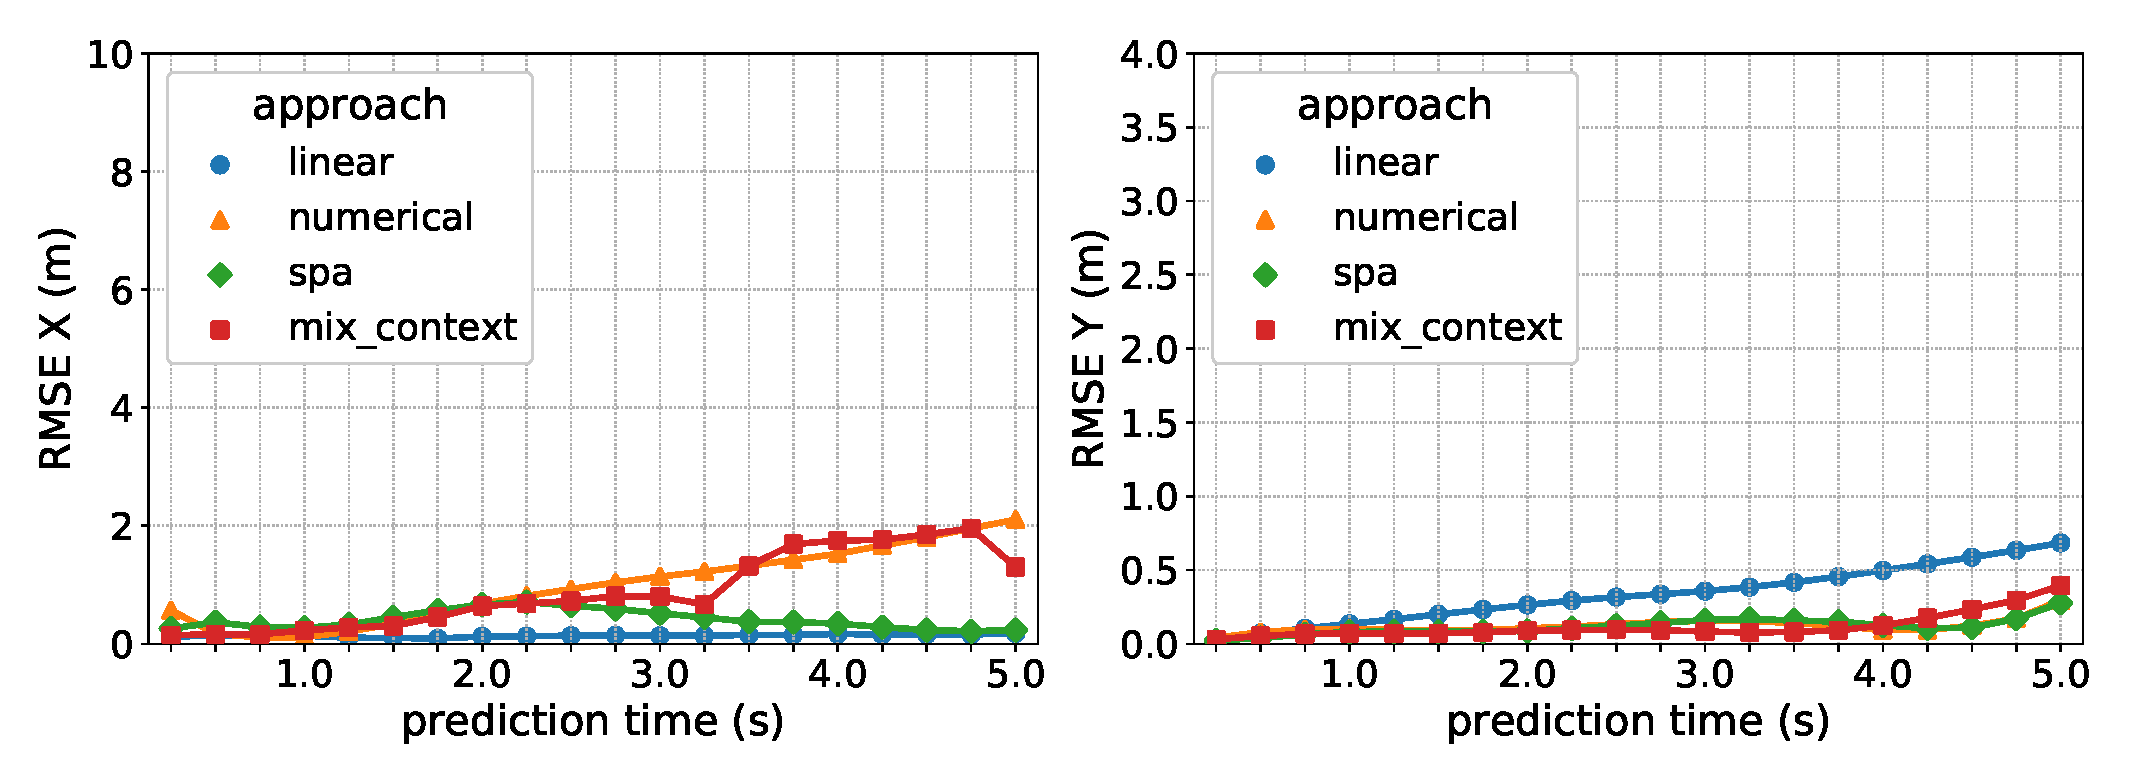
\includegraphics[width=0.5\linewidth]{imgs/mix_vehicle_6.eps}
    }\\
    \subfloat[\label{subfig:mix_vehicle_7}]{%
        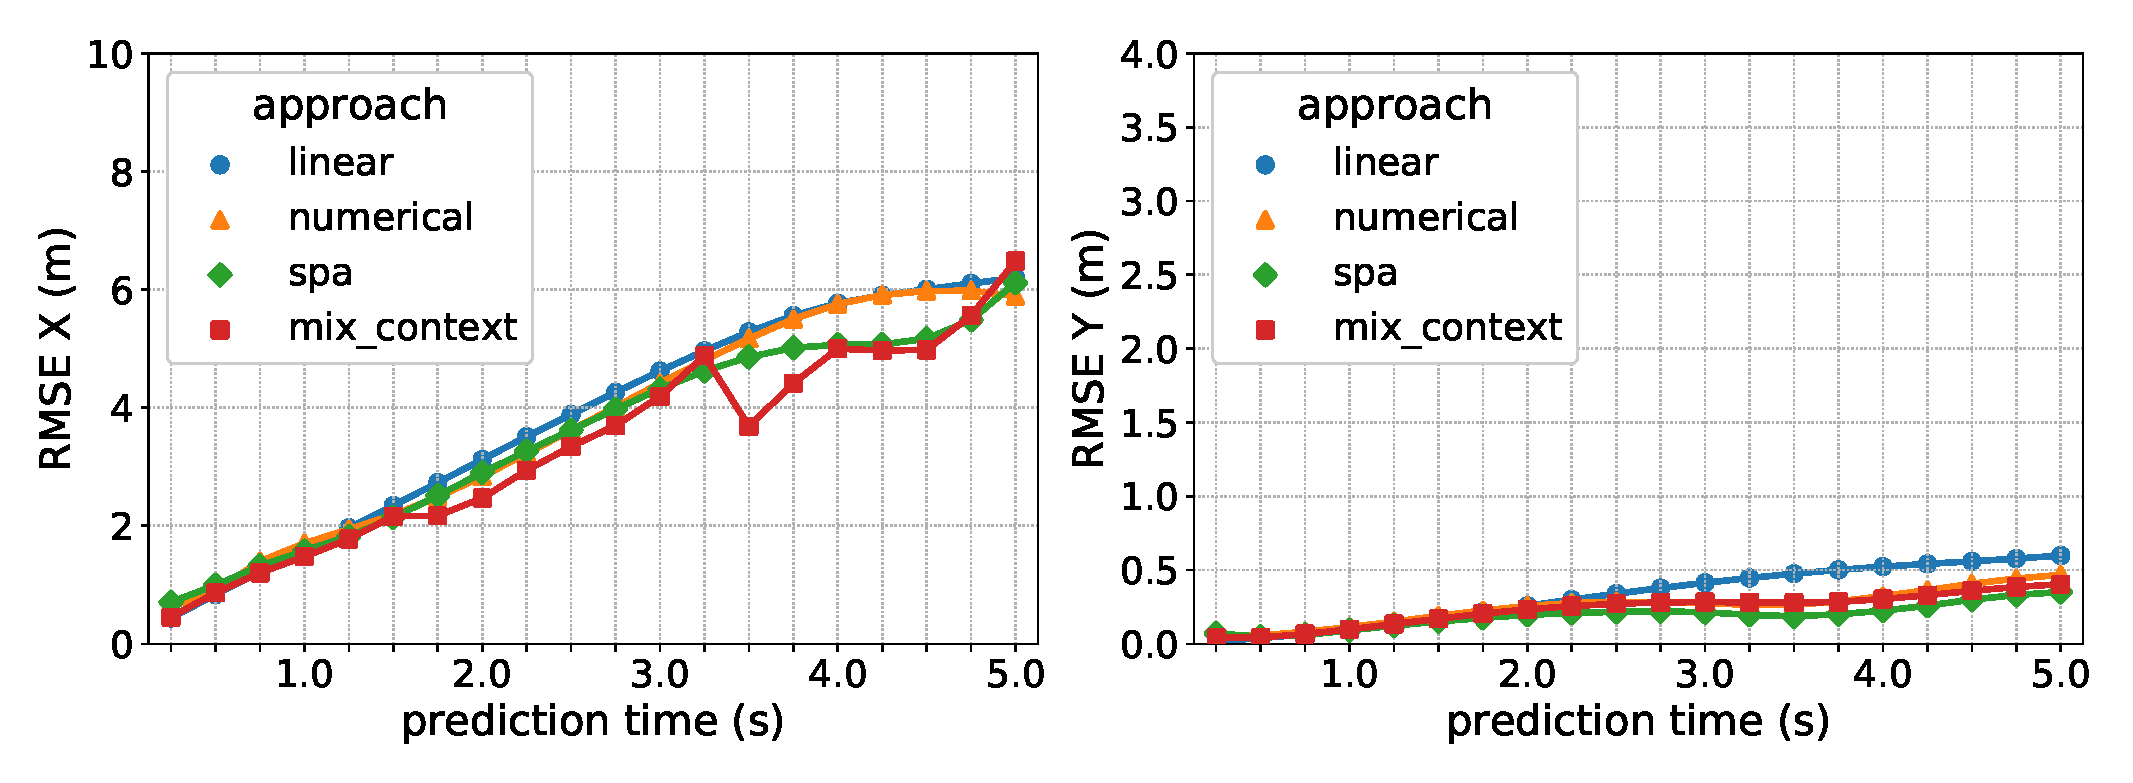
\includegraphics[width=0.5\linewidth]{imgs/mix_vehicle_7.eps}
    }
    \subfloat[\label{subfig:mix_vehicle_8}]{%
        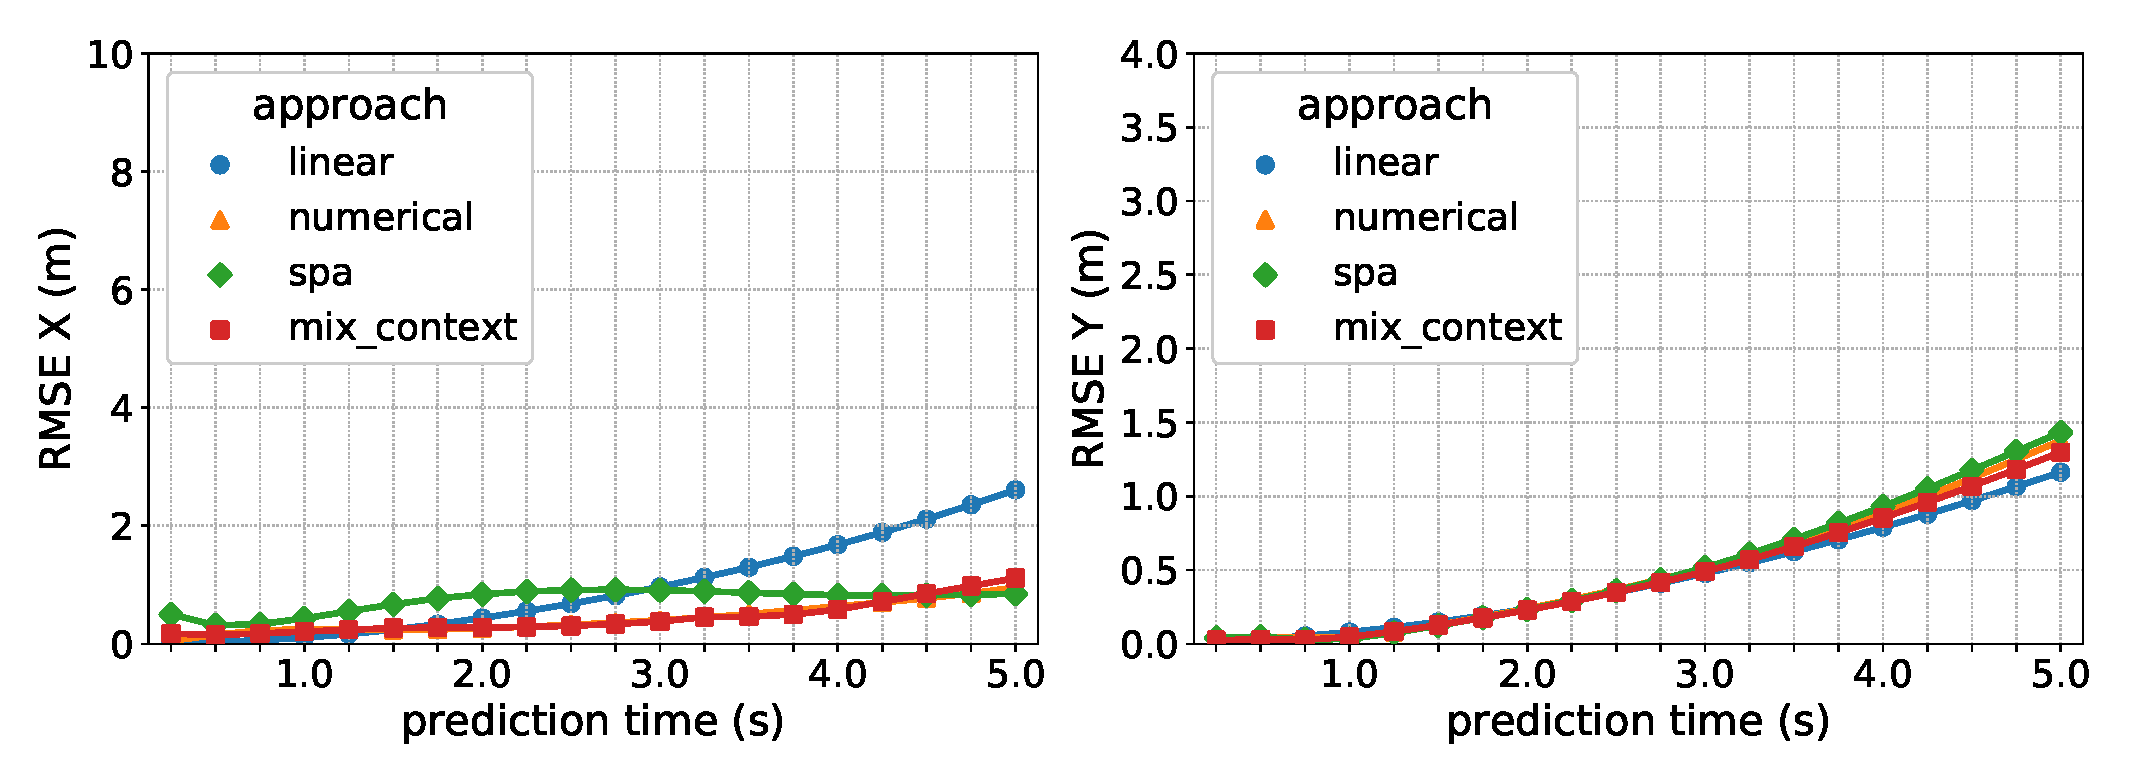
\includegraphics[width=0.5\linewidth]{imgs/mix_vehicle_8.eps}
    }
    \caption{Visualization of the \ac{RMSE} of our mixture-of-experts model on \num{6} different test vehicles in comparison to the input predictors' performance.}
    \label{fig:mix_vehicle_examples}
\end{figure}

To further investigate these results, we evaluate the  model's performance on individual vehicles.
Figure~\ref{fig:mix_vehicle_examples} shows the \ac{RMSE} performance of our mixture-of-experts model in comparison to the individual input predictors on a selection of \num{8} individual test vehicles.
For most of the examples, we observe results similar to the overall, mean performance shown in figure~\ref{fig:mix_vs_other_approaches_over_objects} with the mixture model improving over all individual predictors in $x$-direction and being at least comparable to the best individual predictor in $y$-direction (cf.\ figure~\ref{subfig:mix_vehicle_1},~\ref{subfig:mix_vehicle_3},~\ref{subfig:mix_vehicle_4},~\ref{subfig:mix_vehicle_5}).
However, there are also vehicles such as the one shown in figure~\ref{subfig:mix_vehicle_2}, where we observe improvements of the mixture model over the individual predictors in $y$-direction with no improvements shown in $x$-direction.
For the vehicle shown in figure~\ref{subfig:mix_vehicle_6}, the mixture model does not yield any improvements over the input models in either direction.
For that particular vehicle however, we also observe for both directions, that one of the offline models achieves a remarkably low \ac{RMSE} performance, namely the linear predictor in $x$-direction and the \ac{LSTM} models in $y$-direction, leaving little room for improvement.
However, it would be desirable that our online learning model detects such situations and at least learns to approximate the best available individual offline model.
Figure~\ref{fig:mix_vs_other_approaches_over_objects} shows the \ac{RMSE} performance of our context-sensitive and temporal spreading mixture-of-experts model with \num{2000} neurons on the \num{30} test vehicles in comparison to the individual input predictors.

\section{Summary}
\label{sec:online_learn_summ}

In this chapter, we have extended our work on vehicle trajectory prediction presented in chapter~\ref{chap:behav_pred}.
We have introduced a novel mixture-of-experts online learning model implemented in a spiking neuron substrate employing a simple delta-learning rule to learn to weight different predictor, which have been previously trained offline, at run time.
We presented two variants of this model: one adapting its neural weights simply based on the error between the models predictions and the target vehicle's actual motion and a more advanced version anticipating future motion based on contextual information.
An evaluation of a simplified model variant having access to the error signal, which in a realistic scenario lies in the future, at prediction time showed that the model using contextual information clearly outperforms the context-free version.
Additionally, this simplified model served as an upper bound for the improvement that can be expected from the model having to deal with temporally delayed error signals.
To tackle this issue of delayed error signal, we propose an approach to spread the error signal of earlier prediction times to later time steps.
Our evaluation of this advanced model on real world driving data showed that our approach is able to achieve improvements over the individual offline models already after being presented with only a few example vehicles.
However, the performance gain is not as significant as expected from the experiments with the simplified model variant.
Therefore, there is room for improvement for future work by for instance evaluating how much the model at hand can be further improved by increasing the number of neurons in the context population.
Furthermore, we only investigated one option of contextual information to be used for the mixture model to make predictions, which is in line with the findings of chapter~\ref{chap:behav_pred}.
However, other information, such as the vector representation of the driving scene itself or another more detailed description, could be used as context for the mixture model.
Additionally, we only trained our mixture model on one vehicle at a time.
To allow actual deployment in a driving vehicle, we aim to investigate an advanced version of our approach, which spawns multiple model instantiations to be trained on several vehicles in parallel using shared weights.
Finally, we have not investigated what efficiency benefits could be achieved by deploying our model on specialized neuromorphic hardware.
